\documentclass{article}


\usepackage[utf8]{inputenc}
\usepackage[a4paper, total={6in, 9in}]{geometry}
\usepackage{braket}
\usepackage{xcolor}
\usepackage{amsmath}
\usepackage{amsfonts}
\usepackage{tikz}
\usepackage{svg}
\usepackage{graphicx}
\usepackage{media9}
\usepackage{float}
\usetikzlibrary{calc}
\usepackage{array}
\usepackage[ruled,vlined,linesnumbered]{algorithm2e}

\usepackage[
backend=biber,
style=alphabetic,
sorting=ynt
]{biblatex}



\newcommand{\commentt}[1]{\textcolor{blue}{ \textbf{[COMMENT]} #1}}
\newcommand{\ctt}[1]{\commentt{#1}}
\newcommand{\prb}[1]{ \mathbf{Pr} \left[ {#1} \right]}
\newcommand{\onotation}[1]{\(\mathcal{O} \left( {#1}  \right) \)}
\newcommand{\ona}[1]{\onotation{#1}}
\newcommand{\nvar}[2]{ \( #1_{1}, #1_{2} ... #1_{#2}  \) }
%\newenvironment{proof}[0]{\paragraph{Proof.}}{}
%\newenvironment{remark}[0]{\textit{remark}}{}
\newenvironment{cor}[0]{\paragraph{Corollary.}}{}
\newenvironment{example}[0]{\paragraph{Example.}}{}
%\newenvironment{thm}[0]{\paragraph{Theorem.}}{}
\newtheorem{prop}{Proposition}
\newtheorem{ex}{Exercise}
\newtheorem{sol}{Solution}
\newtheorem{theorem}{Theorem} 		
\newtheorem{thm}{Theorem}[section]
\newtheorem{conj}[thm]{Conjecture} 	
\newtheorem{lemma}[thm]{Lemma}
\newtheorem{corollary}[thm]{Corollary} 
\newtheorem{claim}[thm]{Claim}
\newtheorem{proposition}[thm]{Proposition}
\newtheorem{definition}{Definition} 
\newtheorem{remark}{Remark}
 


% \addbibresource{sample.bib} %Import the bibliography file
\begin{document}    
\maketitle
\section{Correctness - Recitation 2} 
\author{Correctness proofs and computational complexity. }

 
\begin{paragraph}
    Proving algorithms correctness is necessary to guarantee that our code computes its goal for every given input. In that recitation, we will examine several algorithms, analyze theirs running time and memory consumption, and prove they are correct.   
\end{paragraph}


\paragraph{Leading Example.}
Consider \(n\) numbers \(a_1,a_2,....,a_n \in \mathbb{R}\). Given set \(Q\) of \(|Q|\) queries, such each query \(q \in Q\) is a tuple \( (i,j) \in [n] \times [n] \). Write an algorithm that calculates the \(\max_{i\le k\le j}{a_k} \). 

\section{Correctness And Loop Invariant.}

\paragraph{Correctness.} We will say that an algorithm \( \mathcal{A}\) (an ordered set of operations) computes \( f:D_1 \rightarrow D_2 \) if for every \(x \in D_1\) the following equality holds \(f(x) = \mathcal{A}(x)\). Sometimes when it's obvious what is the goal function \(f\), we will abbreviate and say that \( \mathcal{A}\) is correct.       

Examples of functions \(f\) might be: file saving, summing numbers, or posting a message in the forum.  

\paragraph{Loop Invariant.} Loop Invariant is a property that characteristic a loop segment code  and satisfy the following conditions: 
\begin{enumerate}
    \item Initialization. The property holds (even) before the first iteration of the loop.   
    \item Conservation. As long as one performs the loop iterations, the property still holds.
    \item (optional) Termination. Exiting from the loop carrying information.
\end{enumerate}

\paragraph{Example.} Before dealing with the hard problem, let us face the naive algorithm to find the maximum of a given array.

\begin{algorithm}[H]
% \SetAlgoLined
\KwResult{returns the maximum of \(a_1 ... a_n \in \mathbb{R}^n \)  }
 \ \\ 
 \For{ \(i \in [n] \) } { 
        \( j \leftarrow 1 \) \\
        \ \\
        \While{ \(j \le [n] \) and \( a_i \ge a_j \) } {
        \( j \leftarrow j + 1 \)    
        }
        \\
        \ \\ 
        \If { \(j = n+1\) }{
        return \(a_i\)
        }
    } 
return \( \Delta \) 
 \caption{naive maximum alg.}
\end{algorithm}
\paragraph{Claim.} Consider the while loop. The property: \textit{"for every \(j^\prime < j \le n+1 \Rightarrow a_{j^\prime} \le a_i \)"} is a loop invariant that is associated with it. 

\textbf{Proof:} first, the initialization condition holds, as the at the first iteration \(j=1\) and therefore the property is trivial.
Assume by induction, that for every \(m < j\) the property is correct, and consider the \(j\)-th iteration. If back again to line (5), then it means that \( (j-1) < n\) and \( a_{j-1} \le a_{i} \). Combining the above with the induction assumption yields that \(a_i \ge a_{j-1},a_{j-2}, ... a_{1}\).    

\paragraph{Correctness Proof.} Split into cases, First if the algorithm return result at line (9), then due to the loop invariant, combining the fact that \( j = n + 1\), it holds that for every \(j^\prime  \le n < j \Rightarrow a_i \ge a_{j^\prime} \)  i.e \(a_i\) is the maximum of \(a_1, .... a_n \). The second case, in which the algorithm returns \( \Delta \) at line number (10) contradicts the fact that \(n\) is finite, and left as an exercise.  the running time is \( O(n^2) \) and the space consumption is \(O(n)\). 

\paragraph{Loop Invariant In The Cleverer Alg.} Consider now the linear time algorithm:

\begin{algorithm}[H]
% \SetAlgoLined
\KwResult{returns the maximum of \(a_1 ... a_n \in \mathbb{R}^n \)  }
 \ \\ 
 let \(b \leftarrow a_1 \) \\ 
 \ \\ 
 \For{\(i \in [2, n] \) } { 
        \(b \leftarrow \max \left(b, a_i \right) \)
    } 
 return \( b \) 
 \caption{maximum alg.}
\end{algorithm}

What is the Loop Invariant here? \textit{"at the \(i\)-th iteration, \(b = \max{ \{ a_1 ... a_{i-1} \} } \)"}. The proof is almost identical to the naive case.   

\section{Non-Linear Space Complexity Algorithms. }
\paragraph{Sub-Array Maximum.} Consider the leading example; It's easy to write an algorithm that answers the queries at a total time of a \( O\left( |Q| \cdot n \right) \) by answers separately on each query. Can we achieve a better upper bound?

\begin{algbox}{Sub-Array. \(O(n^2)\) space alg.}
\begin{algorithm}[H]
% \SetAlgoLined
\KwResult{print the \( \max{\{ a_i ... a_j \} }\) for each query \((i,j) \in Q \) }
 \ \\ 
 let \(A \leftarrow \mathbb{M}^{n\times n} \) \\ 
 \ \\ 
 \For{\(i \in [n] \) } {
    \( A_{i,i} \leftarrow a_i\)
 }
 \ \\
 \For{ \(k \in [1, n]\) }{
    \For{\(i \in [n] \) } {
        \If{ \(i+k \le n\) }{
        \(A_{i,i+k} \leftarrow \max \left(A_{i,i+k-1}, a_{i+k} \right) \)
        }
    } 
}
\ \\
\For { \( q \in Q \) }{
    \(i,j \leftarrow q \) \\
    print \( A_{i,j}\)
}
\end{algorithm}
\end{algbox}

\paragraph{Claim.} Consider the outer loop at the \(k\)-th step. The following is a loop invariant: \[for \ every \ k^\prime < k ,\ s.t \ i + k^\prime \le n \Rightarrow A_{i,i+k^\prime} = \max{ \{ a_{i}, a_{i+1}, ... ,a_{i + k^\prime} \} }\]  
\textbf{Proof.} The initialization condition trivially holds, assume by induction that \( A_{i,i+k-1} = \max{\{a_i ... a_{i+k-1}\}}\) at beginning of \( k \) iteration. By the fact that \( \max(x,y,z)= \max(\max(x,y),z) \) we get that
\begin{equation*}
\begin{split}
 \max{\{a_1 ... a_{i + k-1}, a_{i+ k} \}} = \max{\{ \max{ \{ a_1 ... a_{i + k-1} \} }, a_{i+ k} \}} =  \max{\{A_{i,i+k-1}, a_{i+ k} \}}
 \end{split}    
 \end{equation*} And the right term is exactly the value which assigned to \(A_{i,i+k}\) in the end of the\(k\)-th iteration. Thus in the beginning of \( k+1 \) iteration the property is still conserved.

\paragraph{ \(O\left(n\log n\right)\) Space Solution.} Example for \(O\left(n\log n + |Q|\log n\right)\) time and \(O\left(n\log n\right)\) space algorithm. Instead of storing the whole matrix, we store only logarithmic number of rows.   

\begin{algbox}{Sub-Array. \(O(n \log n )\) space alg.}
\begin{algorithm}[H]
% \SetAlgoLined
\KwResult{print the \( \max{\{ a_i ... a_j \} }\) for each query \((i,j) \in Q \) }
 \ \\ 
 let \(A \leftarrow \mathbb{M}^{n\times \log n} \) \\ 
 \ \\
 \For{\(i \in [n] \) } {
    \( A_{i,1} \leftarrow a_i\)
 }
 \ \\
 \For{ \(k \in [2,4,..,2^m,...,n]\) }{
    \For{\(i \in [n] \) } {
        \If{ \(i+k \le n\) }{
        \(A_{i,k} \leftarrow \max \left(A_{i,\frac{k}{2}},A_{i+\frac{k}{2}, \frac{k}{2}} \right) \)
        }
    } 
}
\ \\
\For { \( q \in Q \) }{
    \(i,j \leftarrow q \) \\
    decompose \(j - i \) into binary representation \(2^{t_1} + 2^{t_2} + .. +2^{t_l}\) \\
    print \( \max { \{ A_{i,2^{t_1}},A_{i+ 2^{t_1}, 2^{t_2} }, ... , A_{i+ 2^{t_1} + 2^{t_2} +.. 2^{t_{l-1}}, 2^{t_l}} \} }\)
}
\end{algorithm}
\end{algbox}



\newpage
\section{Recursive Analysis - Recitation 3} 
\author{Master theorem and recursive trees.}

 
\begin{paragraph}
    One of the standard methods to analyze the running time of algorithms is to express recursively the number of operations that are made. In the following recitation, we will review the techniques to handle such formulation (solve or bound).  
\end{paragraph}


\section{Bounding recursive functions by hands.} Our primary tool to handle recursive relation is the Master Theorem, which was proved in the lecture. As we would like to have a more solid grasp, let's return on the calculation in the proof over a specific case. 
Assume that your algorithm analysis has brought the following recursive relation:
\begin{enumerate}
    \item \textbf{Example.} \( T\left(n\right)  = \left\{ \begin{array}{rcl}
& 4T\left(\frac{n}{2}\right)+c\cdot n & \mbox{for }  n > 1  \\
& 1 & \mbox{else}  
\end{array}\right. \). Thus, the running time is given by \begin{equation*}
    \begin{split}
 & T\left(n\right)  = 4T\left(\frac{n}{2}\right)+c\cdot n=  4\cdot4T\left(\frac{n}{4}\right)+4c\cdot\frac{n}{2}+c\cdot n = ... = \\ & \overset{\text{\textcolor{red}{critical}}}{\overbrace{4^{h}T(1)}} + c\cdot n\left(1+\frac{4}{2}+\left(\frac{4}{2}\right)^{2}...+\left(\frac{4}{2}\right)^{h-1}\right) = 4^{h} + c\cdot n\cdot\frac{2^{h}-1}{2-1}
    \end{split}
\end{equation*}
We will call the number of iteration till the stopping condition the recursion height, and we will denote it by \(h\) . What should be the recursion height? \( 2^{h} = n \Rightarrow h =\log\left(n\right) \). So in total we get that the algorithm running time equals \( \Theta\left(n^2\right)\). 

\textbf{Question}, Why is the term \( 4^{h} T(1) \) so critical? Consider the case \(T\left(n\right) =  4T\left(\frac{n}{2}\right) + c \) .One popular mistake is to forget the final term, which yields a linear solution \( \Theta(n)\) (instead of quadric \( \Theta(n^2)\)).   

    \item \textbf{Example.} \( T\left(n\right) & = \left\{ \begin{array}{rcl}
& 3T\left(\frac{n}{2}\right) + c\cdot n & \mbox{for }  n > 1  \\
& 1 & \mbox{else}  
\end{array}\right. \), and then the expanding yields: 
\begin{equation*}
    \begin{split}
        T\left(n\right) & = 3T\left(\frac{n}{2}\right) + c\cdot n = 3^2 T\left(\frac{n}{2^2}\right) + \frac{3}{2}cn + c\cdot n =  \overset{\text{\textcolor{red}{critical}}}{\overbrace{3^{h}T(1)}} + cn\left(1 + \frac{3}{2} + \left(\frac{3}{2}\right)^2 + ...  + \left(\frac{3}{2}\right)^{h-1} \right) \\
        & h = \log_{2}\left(n\right) \Rightarrow T\left(n\right) = 3^{h}T(1) + c\cdot \textcolor{red}{n}\cdot \left(\left(\frac{3}{\textcolor{red}{2}}\right)^{\log_{2}{n}}\right) / \left(\frac{3}{2} - 1\right) = \theta \left( 3^{\log_{2}(n)} \right) =  \theta \left( n^{\log 3} \right)  
    \end{split}
\end{equation*}
where \(n^{\log 3}  \sim n^{1.58} < n^2 \).
\end{enumerate}



\section{Master Theorem, one Theorem to bound them all. }
As you might already notice, the same pattern has been used to bound both algorithms. The master theorem is the result of the recursive expansion. it classifies recursive functions at the form of \(T\left(n\right) = a\cdot T\left( \frac{n}{b} \right) + f\left(n\right) \), for positive function \(f : \mathbb{N} \rightarrow \mathbb{R}^{+} \).       

\begin{defbox}{Master Theorem, simple version.} First, Consider the case that \(f = n^c\). Let \( a \ge 1, b > 1\) and \( c \ge 0 \). then: 
\begin{enumerate}
    \item if \(\frac{a}{b^c} < 1 \) then \( T\left(n\right) = \Theta \left( n^c \right) \) \ \ \ \textbf{(\(f\) wins)}.
    \item if \(\frac{a}{b^c} = 1 \) then \( T\left(n\right) = \Theta \left( n^c \log_{b} \left(n\right) \right) \).
    \item if \(\frac{a}{b^c} > 1 \) then \( T\left(n\right) = \Theta \left( n^{\log_{b} \left(a\right)} \right) \) \ \ \ \textbf{(\(f\) loose)}.
  \end{enumerate}
\end{defbox}

\paragraph{Example.}  \( T\left(n\right)  =4T\left(\frac{n}{2}\right)+d\cdot n \Rightarrow
T\left(n\right) = \Theta\left(n^2\right)\) according to case (3). And \(T\left(n\right) & = 3T\left(\frac{n}{2}\right) + d\cdot n \Rightarrow T\left(n\right) = \Theta \left( n^{\log_{2}\left(3\right)}\right)\)
also due to case (3).

\begin{defbox}{Master Theorem, strong version.} 
Now, let's generalize the simple version for arbitrary positive \(f\) and let \( a \ge 1, b > 1\). 

\newcommand{\logab}{\log_{b} \left(a\right)}

\begin{enumerate}
    \item if  \(f\left(n\right) = O \left( n^{\logab - \varepsilon }\right)\) for some \( \varepsilon > 0 \) then \( T\left(n\right) = \theta \left( n^{\logab} \right) \) \ \ \ \textbf{(\(f\) loose)}.
    
    \item if  \(f\left(n\right) = \Theta \left( n^{\logab} \right) \) then \( T\left(n\right) = \Theta \left( n^{\logab}  \log\left(n\right)\right) \)
    
    \item if there exist \(\varepsilon >0 ,c<1\) and \(n_0 \in \mathbb{N} \) such that  \(f\left(n\right) = \Omega \left( n^{\logab + \varepsilon }\right)\) and for every \( n > n_0 \) \(a \cdot f\left( \frac{n}{b} \right) \le c f\left(n\right)\)  then \( T\left(n\right) = \theta \left( f\left(n\right) \right) \) \ \ \ \textbf{(\(f\) wins)}.
    
\end{enumerate}
\end{defbox}
\newcommand{\TT}[2]{#1 T\left(\frac{n}{#2}\right)}

\paragraph{Examples}
\begin{enumerate}
    \item \( T\left(n\right) =  T\left(\frac{2n}{3}\right) + 1 \rightarrow f\left(n\right) = 1 =\Theta \left( n^{\log_{\frac{3}{2}} \left(1\right)}\right)\) matches the second case. i.e  \( T\left(n\right) = \Theta \left( n^{\log_{\frac{3}{2}} \left(1\right)}\log n \right)\).
    
    \item \( T\left(n\right) = \TT{3}{4} + n\log n \rightarrow f\left(n\right) = \Omega\left( n^{\log_{4}\left(3\right) + \varepsilon}  \right) \) and notice that \( f\left( a\frac{n}{b}\right) = \frac{3n}{4}\log\left(\frac{3n}{4}\right)\) . Thus, it's matching to the third case. \(\Rightarrow T\left(n\right) = \Theta\left(n\log n\right)\).
    
    \item \(T\left(n\right) = 3T\left( n^{\frac{1}{3}}\right) + \log\log n\). let \( m = \log n \Rightarrow T\left( n\right) = T \left(2^m \right) = 3T\left(2^{\frac{m}{3}} \right) + \log m\). denote by \(S = S\left(m\right) = T\left(2^m\right) \rightarrow S\left(m\right) = 3T\left(2^{\frac{m}{3}} \right) + \log m = 3S\left(\frac{m}{3} \right) + \log m\). And by the fact that \(\log m = O\left(m^{\log_{3}\left(3\right)-\varepsilon} \right) \rightarrow T\left(n\right) = T\left(2^m\right) = S\left(m\right) = \Theta\left(m\right) = \Theta\left( \log(n)\right) \).  
\end{enumerate}


\section{Recursive trees.}
There are still cases which aren't treated by the \textit{Master Theorem}. For example consider the function \(T\left(n\right) = 2T\left(\frac{n}{2}\right) + n\log n \). Note, that \(f = \Omega\left( n^{\log_{b}(a)} \right) = \Omega\left(n\right)\). Yet for every \( \varepsilon > 0 \Rightarrow f = n\log n = O\left( n^{1+\varepsilon} \right) \) therefore the third case  doesn't hold. How can such cases still be analyzed? 

\paragraph{Recursive trees Recipe}
    \begin{enumerate}
        \item draw the computation tree, and calculate it's height. in our case, \( h = \log n \).
        \item calculate the work which done over node at the \(k\)-th level, and the number of nodes in each level. in our case, there are \(2^k\) nodes and over each we perform \(f(n) = \frac{n}{2^k} \log\left( \frac{n}{2^k}\right)\) operations. 
        \item sum up the work of the \(k\)-th level.
        \item finally, the total time is the summation over all the \( k \in [h]\) levels. 
    \end{enumerate}
applying the above, yields 
\begin{equation*} 
\begin{split} 
T\left(n\right) & =  \sum_{k=1}^{\log{n}}{n\cdot\log \left( \frac{n}{2^k}\right)} = n\sum_{k=1}^{\log{n}}{ \left( \log n - \log 2^k \right) } 
  = n\sum_{k=1}^{\log{n}}{ \left( \log n - k \right) } = \\ & = \Theta \left( n \log^2 \left(n\right)  \right) 
\end{split}
\end{equation*}
za
\pzaaragraph{Example.} Consider merge sort variation such that instead of splitting the array into two equals parts it's split them into different size arrays. The first one contains \( \frac{n}{10} \) elements while second contains the others \( \frac{9n}{10}\) elements.

\begin{algbox}{non-equal-merge alg.}
\begin{algorithm}[H]
\SetAlgoLined
\KwResult{returns the sorted permutation of \(x_1 ... x_n \in \mathbb{R}^n \)  }
 \ \\ 
 \If{ \(n \le 10 \) }
    { return bubble-sort \( (x_1 ... x_n)\) } 
 \ \\ 
 
 \Else {
 define \(S_{l} \leftarrow x_1 ... x_{\frac{n}{10}-2}, x_{\frac{n}{10}-1} \) \\
 define \(S_{r} \leftarrow   x_{\frac{n}{10}},x_{\frac{n}{10}+1} ...,x_n \) \\
 \ \\ 
 \( R_l \leftarrow \) non-equal-merge\( \left( S_l \right) \) \\ 
 \( R_r \leftarrow \) non-equal-merge\( \left( S_r \right) \) \\
 \ \\
 return Merge(\(R_l, R_r\))
  
 }
\end{algorithm}
\end{algbox}
Note, that the master theorem achieves an upper bound, 
\begin{equation*}
    \begin{split}
        T\left(n\right) & = n +  T\left(\frac{n}{10}\right) + T\left(\frac{9n}{10}\right) \le n +  2 T\left(\frac{9n}{10}\right) \Rightarrow T\left(n\right) = O \left( n^{\log_{\frac{10}{9}}\left(2\right)} \right) \sim O \left( n^{ 6 } \right)  
    \end{split}
\end{equation*}
Yet, that bound is far from been tight. Let's try to count the operations for each node. Let's try another direction. 
\paragraph{Claim.} Let \(n_i\) be the size of the subset which is processed at the \(i\)-th node. Then for every \(k\):
\begin{equation*}
    \sum_{i \in \text{k level}}{n_i} \le n
\end{equation*}
 \textbf{Proof}. Assuming otherwise implies that there exist index \(j\) such that \(x_j\) appear in at least two different nodes in the same level, denote them by \(u,v\). As they both are in the same level, non of them can be ancestor of the other. denote by \(m \in \mathbb{N}\) the input size of the sub array which is processed by the the lowest common ancestor of \(u\) and \(v\), and by \(j^\prime \in [m]\) the position of \(x_j\) in that sub array. By the definition of the algorithm it steams that \(j^\prime < \frac{m}{10} \) and \(j^\prime \ge \frac{m}{10}\). contradiction.  


 The height of the tree is bounded by \( \log_{\frac{9}{10}} \left(n\right) \). Therefore the total work equals \( \Theta \left( n\log n \right) \).    

Thus, the total running time equals to:
\begin{equation*}
    T(n) = \sum_{k \in \text{levels}}{\sum_{i \in \text{k level}}{f\left(n_i\right)}} = \sum_{k \in \text{levels}}{\sum_{i \in \text{k level}}{n_i}} \le n\log n  
\end{equation*}



\section{Appendix. Recursive Functions In Computer Science. (Optional)}

\ctt{The current section repeats over part of the content above as it was designed to be self-contained. Also, notice that this part is considered as optional material and you are not required to remember the following algorithms for the final exam. Its primary goal is to expose you to "strange" running times. }


\paragraph{Leading Example. numbers multiplication}
Let \(x,y\) be an \(n\)'th digits numbers over \( \mathbb{F}^{n}_{2} \). It's known that summing such a pair requires a linear number of operations. Write an algorithm that calculates the multiplication \(x\cdot y\). 

\paragraph{Example. Long multiplication.} 
To understand the real power of the dividing and conquer method, let's first examine the known solution from elementary school.  In that technics, we calculate the power order and the value of the digit separately and sum up the results at the end. Formally: \(x \leftarrow \sum_{i=0}^{n}{x_{i}2^{i}}\) Thus, \[ x\cdot y =\left( \sum_{i=0}^{n}{x_{i}2^{i}} \right) \left( \sum_{i=0}^{n}{y_{i}2^{i}} \right) =  \sum_{i,j \in [n]\times[n] }{ x_{i}y_{j}2^{i+j} }\] the above is a sum up over \(n^2\) numbers, each at length \(n\) and therefore the total running time of the algorithm is bounded by \( \theta(n^3) \). \ctt{ notice that adding \(1\) to \(1111111111...1\) requires \(O(n)\) }.

\paragraph{Example. Recursive Approach.} We could split \(x\) into the pair \(x_{l}, x_{r}\) such that \(x = x_{l} + 2^{\frac{n}{2}}x_{r} \). Then the multiplication of two \(n\)-long numbers will be reduced to sum up over multiplication of a quartet. Each at length \(\frac{n}{2}\). Thus, the running time is given by \begin{equation*}
    \begin{split}
 x\cdot y & = \left(x_{l} + 2^{\frac{n}{2}}x_{r}\right)\left(y_{l} + 2^{\frac{n}{2}}y_{r}\right) = x_{l}y_{l} + 2^{\frac{n}{2}} \left( x_{l}y_{r} + x_{r}y_{l} \right) + 2^{n}x_{r}y_{r} \\ &  \Rightarrow T\left(n\right)  =4T\left(\frac{n}{2}\right)+c\cdot n=4\cdot4T\left(\frac{n}{4}\right)+4c\cdot\frac{n}{2}+c\cdot n = ... = \\ & c\cdot n\left(1+\frac{4}{2}+\left(\frac{4}{2}\right)^{2}...+\left(\frac{4}{2}\right)^{h-1}\right) + 4^{h}T(1) = n^{2} + c\cdot n\cdot\frac{2^{h}-1}{2-1}
    \end{split}
\end{equation*}
We will call the number of iteration till the stopping condition the recursion height, and we will denote it by \(h\) . What should be the recursion height? \( 2^{h} = n \Rightarrow h =\log\left(n\right) \). So in total we get that multiplication could be achieved by performs \( \Theta\left(n^2\right)\) operations. 
\paragraph{Example. Karatsuba algorithm.} Many years it's was believed that multiplication can't done by less then \( \Omega \left( n^2 \right) \) time; until Karatsuba found the following algorithm. denote by \begin{equation*}
z_0, z_1, z_2 \leftarrow x_{l}y_{r}, x_{l}y_{r} + x_{r}y_{l}, x_{r}y_{r}
\end{equation*}Notice that \( z_1 = \left(x_{l}+x_{r}\right)\left(y_{l}+y_{r}\right) - z_{0} -z_{1} \). summarize the above yields the following pseudo code. 

\begin{algbox}{Karatsuba alg.}
\begin{algorithm}[H]
\SetAlgoLined
\KwResult{returns the multiplication \(x\cdot y\) where \(x,y \in \mathbb{F}^{n}_{2}\) }
 \ \\ 
 \If{ \(x,y \in \mathbb{F}_{2}\) }
    { return \(x \cdot y\) } 
 \ \\ 
 
 \Else {
 define \(x_{l} , x_{r} \leftarrow x \) and \(y_{l} , y_{r} \leftarrow x \) \ \ \ \ \ // \( O \left(n\right) \). \\ 
 \ \\ 
 calculate \(z_0 \leftarrow \text{Karatsuba}\left(x_{l},y_{l}\right)\) \\
 \ \ \ \ \ \ \ \ \ \ \ \ \(z_2 \leftarrow \text{Karatsuba}\left(x_{r},y_{r}\right)\) \\ 
 \ \ \ \ \ \ \ \ \ \ \ \ \(z_1 \leftarrow \text{Karatsuba}\left(x_{r} + x_{l} ,y_{l} + y_{r} \right) - z_0 - z_2 \) \\ 
 \ \\
 return \(z_0 + 2^{\frac{n}{2}}z_1 + 2^{n}z_2\) \ \ \ \ \  // \( O \left(n\right) \). 
 }
\end{algorithm}
\end{algbox}
Let's analyze the running time of the algorithm above, assume that \(n = 2^{m}\) and then the recursive relation is 
\begin{equation*}
    \begin{split}
        T\left(n\right) & = 3T\left(\frac{n}{2}\right) + c\cdot n = 3^2 T\left(\frac{n}{2^2}\right) + \frac{3}{2}cn + c\cdot n = cn\left(1 + \frac{3}{2} + \left(\frac{3}{2}\right)^2 + ...  + \left(\frac{3}{2}\right)^{h-1} \right) + ) + 3^{h}T(1) \\
        & h = \log_{2}\left(n\right) \Rightarrow T\left(n\right) = n^{\log_{2}{3}} +  c\cdot \textcolor{red}{n}\cdot \left(\left(\frac{3}{\textcolor{red}{2}}\right)^{\log_{2}{n}}\right) / \left(\frac{3}{2} - 1\right) = \theta \left( 3^{\log_{2}(n)} \right) =  \theta \left( n^{\log 3} \right)  
    \end{split}
\end{equation*}
where \(n^{\log 3}  \sim n^{1.58} < n^2 \).



\newpage\section{Heaps - Recitation 4} 
\author{Correctness, Loop Invariant And Heaps.}


%\begin{paragraph}
  Apart from quantifying the resource requirement of our algorithms, we are also interested in proving that they indeed work. In this Recitation, we will demonstrate how to prove correctness via the notation of loop invariant. In addition, we will present the first (non-trivial) data structure in the course and prove that it allows us to compute the maximum efficiently.

%\end{paragraph}


\subsection*{Correctness And Loop Invariant.}
In this course, any algorithm is defined relative to a task/problem/function, And it will be said correctly if, for any input, it computes desirable output. For example, suppose that our task is to extract the maximum element from a given array. 
So the input space is all the arrays of numbers, and proving that a given algorithm is correct requires proving that the algorithm's output is the maximal number for an arbitrary array. Formally:  
\begin{defbox}{Correctness.}
We will say that an algorithm \( \mathcal{A}\) (an ordered set of operations) computes \( f:D_1 \rightarrow D_2 \) if for every \(x \in D_1 \Rightarrow f(x) = \mathcal{A}(x)\). Sometimes when it's obvious what is the goal function \(f\), we will abbreviate and say that \( \mathcal{A}\) is correct.       
\end{defbox}
\paragraph{}
Other functions \(f\) might be including any computation task: file saving, summing numbers, posting a message in the forum, etc. Let's dive back into the maximum extraction problem and see how one should prove correctness in practice.     
\paragraph{Task: Maximum Finding.} \textit{Given $n\in \mathbb{N}$ numbers $a_1, a_2, \cdots a_n \in \mathbb{R}$ write an Algorithm that returns their maximum.} 

Consider the following suggestion. How would you prove it correct?  
\begin{algbox}{Maximum finding.}
\begin{algorithm*}[H]
% \SetAlgoLined
 \SetKwInOut{Input}{input}
 \Input{ Array  $ a_1, a_2, .. a_n $  }
 let \(b \leftarrow a_1 \) \\ 
 \For{\(i \in [2, n] \) } { 
        \(b \leftarrow \max \left(b, a_i \right) \)
    } 
 return \( b \) 
 %\caption{maximum alg.}
\end{algorithm*}
\end{algbox}
Usually, it will be convenient to divide the algorithms into subsections and then characterize and prove their correctness separately. One primary technique is using the notation of Loop Invariant. Loop Invariant is a property that is characteristic of a loop segment code  and satisfies the following conditions:
\begin{defbox}{Loop Invariant.} 
\begin{enumerate}
  \item Initialization. The property holds (even) before the first iteration of the loop.    
    \item Conservation. As long as one performs the loop iterations, the property still holds.
    \item Termination. Exiting from the loop carrying information.
\end{enumerate}
\end{defbox}

Let's denote by $b^{(i)}$ the value of $b$ at line number $2$ at the $i$th iteration for $i\ge2$ and define $b^{(1)}$ to be its value in its initialization. What is the Loop Invariant here? \textbf{Claim.} \textit{"at the \(i\)-th iteration, $b^{(i)} = \max{ \{ a_1 ... a_{i} \} } $"}. 
\paragraph{Proof.} Initialization, clearly, $ b^{(1)} = a_{1} = \max{ \{ a_1 \} } $. Conservation, by induction, we have the base case from the initialization part, assume the correctness of the claim for any $i^\prime < i$, and consider the $i$th iteration (of course, assume that $i<n$). Then:  
\begin{equation*}
  \begin{split}
b^{(i)} = \max{ \{ b^{(i-1)}, a_{i} \} } = \max{ \{ \max{ \{ a_1, .. a_{i-2}, a_{i-1} \} }, a_{i} \} } = \max{ \{  a_{1}, .. a_{i} \} }
  \end{split}
\end{equation*} 
And that completes the Conservation part. Termination, followed by the conservation, at the $n$ iteration, $b^{(i)}$ is seted to $\max{ \{ a_1 ,a_2 .. a_n  \}}$. 

\paragraph{Task: Element finding.}  \textit{Given $n\in \mathbb{N}$ numbers $a_1, a_2, \cdots a_n \in \mathbb{R}$ and additional number $x \in \mathbb{R}$ write an Algorithm that returns $i$ s.t $a_{i} = x$ if there exists such $i$ and} False \textit{otherwise.} 

\begin{algbox}{Element finding.}
\begin{algorithm}[H]
\SetKwInOut{Input}{input}
 \Input{ Array  $ a_1, a_2, .. a_n $  }
% \SetAlgoLined
 \For{ \(i \in [n] \) } { 
	\If { \(a_{i} = x\) }{
	  return \(i, a_{i}\)
        }
    } 
    return False 
\end{algorithm}
\end{algbox}
\paragraph{Correctness Proof.} First, let's prove the following loop invariant. 
\subparagraph{Claim} \textit{Suppose that the running of the algorithm reached the i-th iteration, then $x \notin \{ a_{1} .. a_{i-1} \}$.} 
\textbf{Proof.} Initialization, for $i=1$ the claim is trivial. Let's use that as the induction base case for proving Conservation. Assume the correctness of the claim for any $i^{\prime} < i$. And consider the $i$th iteration. By the induction assumption, we have that $x \notin \{a_1 .. a_{i-2} \} $, and by the fact that we reached the $i$th iteration, we have that in the $i-1$ iteration, at the line (2) the conditional weren't satisfied (otherwise, the function would return at line (3) namely $x \neq a_{i-1}$. Hence, it follows that $ x \notin \{ a_1, a_2 .. a_{i-2}, a_{i-1} \} $.     
  \subparagraph{} Separate to cases. First, consider the case that given the input $a_1 .. a_n$, the algorithm return False. In this case, we have by the termination property that $x \notin \{ a_1 .. a_n \} $. Now, Suppose that the algorithm returns the pair $\left( i, x \right)$, then it means that the conditional at the line (2) was satisfied at the $i$th iteration. So, indeed $a_{i} = x$, and the algorithm returns the expected output.        


  \newpage
\subsection*{Heaps.}
  \paragraph{Task: The Superpharm Problem. (Motivation for Heaps) }\textit{You are requested to maintain a pharmacy line. In each turn, you get one of the following queries, either a new customer enters the shop, or the pharmacist requests the next person to stand in front. In addition, different customers have different priorities, So you are asked to guarantee that in each turn, the person with the height priority will be at the front.}

Before we consider a sophisticated solution, What is the running time for the naive solution? (maintaining the line as a linear array) ($\sim O\left( n^2 \right)$).

Heaps are structures that enable computing the maximum efficiency in addition to supporting adding and removing elements.
We have seen in the Lecture that no Algorithm can compute the $\max$ function with less than $n-1$ comparisons. So our solution above is indeed the best we could expect for. The same is true for the element-finding problem. Yet, we saw that if we are interested in storing the numbers, then, by keeping them according to sorted order, we could compute each query in logarithmic time via binary search. That raises the question, is it possible to have a similar result regarding the max problem?

\begin{defbox}{Heap}
  Let $n \in \mathbb{N}$ and consider the sequence $H = H_{1}, H_{2} \cdots H_{n} \in \mathbb{R} \left( * \right)$. we will say that $H$ is a Heap if for every $i \in [n]$ we have that: $H_{i} \le H_{2i}, H_{2i + 1}$ when we think of the value at indices greater than $n$ as $H_{i>n} = -\infty$. 
  \begin{equation*}
    \begin{split}
      \Leftrightarrow
    \end{split}
  \end{equation*}
  That definition is equivalent to the following recursive definition: Consider a binary tree in that we associate a number for each node. Then, we will say that this binary tree is a heap if the root's value is lower than its sons' values, and each subtree defined by its children is also a heap. 
\end{defbox}


    % Drawing a graph using the PG 3.0 graphdrawing library
% Author: Mark Wibrow
%\documentclass[tikz,border=10pt]{article}
%\usepackage{tikz}
%\usetikzlibrary{positioning}
%\begin{document}

\tikzset{%
  every neuron/.style={
    circle,
    draw,
    %fill=black,
    radius=0.05mm
  },
  neuron missing/.style={
    draw=none,
    scale=2,
    text height=0.25cm,
    execute at begin node=\color{black}$\vdots$
  },
}

\begin{tikzpicture}
    \node [every  neuron ] (v-1) at ( 0.0 ,-0) { $1$  };\node [every  neuron ] (v-2) at ( 0.0 ,-1) { $2$  };\node [every  neuron ] (v-3) at ( 4.0 ,-1) { $3$  };\node [every  neuron ] (v-4) at ( 0.0 ,-2) { $4$  };\node [every  neuron ] (v-5) at ( 2.0 ,-2) { $5$  };\node [every  neuron ] (v-6) at ( 4.0 ,-2) { $6$  };\node [every  neuron ] (v-7) at ( 6.0 ,-2) { $7$  };\node [every  neuron ] (v-8) at ( 0.0 ,-3) { $8$  };\node [every  neuron ] (v-9) at ( 1.0 ,-3) { $9$  };\node [every  neuron ] (v-10) at ( 2.0 ,-3) { $10$  };\node [every  neuron ] (v-11) at ( 3.0 ,-3) { $11$  };\node [every  neuron ] (v-12) at ( 4.0 ,-3) { $12$  };\node [every  neuron ] (v-13) at ( 5.0 ,-3) { $13$  };\node [every  neuron ] (v-14) at ( 6.0 ,-3) { $14$  };\node [every  neuron ] (v-15) at ( 7.0 ,-3) { $15$  };\draw [->] (v-1) -- (v-2);\draw [->] (v-1) -- (v-3);\draw [->] (v-2) -- (v-4);\draw [->] (v-2) -- (v-5);\draw [->] (v-3) -- (v-6);\draw [->] (v-3) -- (v-7);\draw [->] (v-4) -- (v-8);\draw [->] (v-4) -- (v-9);\draw [->] (v-5) -- (v-10);\draw [->] (v-5) -- (v-11);\draw [->] (v-6) -- (v-12);\draw [->] (v-6) -- (v-13);\draw [->] (v-7) -- (v-14);\draw [->] (v-7) -- (v-15);\end{tikzpicture}
\paragraph{Checking vital signs.}Are the following sequences are heaps? 
\begin{enumerate}
  \item 1,2,3,4,5,6,7,8,9,10 (Y)
  \item 1,1,1,1,1,1,1,1,1,1  (Y)
  \item 1,4,3,2,7,8,9,10     (N)
  \item 1,4,2,5,6,3	     (Y)
\end{enumerate}
\begin{figure}[h]
  \centering
  \begin{subfigure}[b]{0.3\textwidth}
	
    % Drawing a graph using the PG 3.0 graphdrawing library
% Author: Mark Wibrow
%\documentclass[tikz,border=10pt]{article}
%\usepackage{tikz}
%\usetikzlibrary{positioning}
%\begin{document}

\tikzset{%
  every neuron/.style={
    circle,
    draw,
    %fill=black,
    radius=0.05mm
  },
  neuron missing/.style={
    draw=none,
    scale=2,
    text height=0.25cm,
    execute at begin node=\color{black}$\vdots$
  },
}

\begin{tikzpicture}
    \node [every  neuron ] (v-1) at ( 0.0 ,-0) { $1$  };\node [every  neuron ] (v-2) at ( 0.0 ,-1) { $1$  };\node [every  neuron ] (v-3) at ( 2.5 ,-1) { $1$  };\node [every  neuron ] (v-4) at ( 0.0 ,-2) { $1$  };\node [every  neuron ] (v-5) at ( 1.25 ,-2) { $1$  };\node [every  neuron ] (v-6) at ( 2.5 ,-2) { $1$  };\node [every  neuron ] (v-7) at ( 3.75 ,-2) { $1$  };\node [every  neuron ] (v-8) at ( 0.0 ,-3) { $1$  };\node [every  neuron ] (v-9) at ( 0.625 ,-3) { $1$  };\draw [->] (v-1) -- (v-2);\draw [->] (v-1) -- (v-3);\draw [->] (v-2) -- (v-4);\draw [->] (v-2) -- (v-5);\draw [->] (v-3) -- (v-6);\draw [->] (v-3) -- (v-7);\draw [->] (v-4) -- (v-8);\draw [->] (v-4) -- (v-9);\end{tikzpicture}
  \end{subfigure}
\begin{subfigure}[b]{0.3\textwidth}
	
    % Drawing a graph using the PG 3.0 graphdrawing library
% Author: Mark Wibrow
%\documentclass[tikz,border=10pt]{article}
%\usepackage{tikz}
%\usetikzlibrary{positioning}
%\begin{document}

\tikzset{%
  every neuron/.style={
    circle,
    draw,
    %fill=black,
    radius=0.05mm
  },
  neuron missing/.style={
    draw=none,
    scale=2,
    text height=0.25cm,
    execute at begin node=\color{black}$\vdots$
  },
}

\begin{tikzpicture}
    \node [every  neuron ] (v-1) at ( 0.0 ,-0) { $1$  };\node [every  neuron, fill=black,  text=white, draw=black ] (v-2) at ( 0.0 ,-1) { $4$  };\node [every  neuron ] (v-3) at ( 2.0 ,-1) { $3$  };\node [every  neuron ] (v-4) at ( 0.0 ,-2) { $2$  };\node [every  neuron ] (v-5) at ( 1.0 ,-2) { $7$  };\node [every  neuron ] (v-6) at ( 2.0 ,-2) { $8$  };\node [every  neuron ] (v-7) at ( 3.0 ,-2) { $9$  };\draw [->] (v-1) -- (v-2);\draw [->] (v-1) -- (v-3);\draw [->] (v-2) -- (v-4);\draw [->] (v-2) -- (v-5);\draw [->] (v-3) -- (v-6);\draw [->] (v-3) -- (v-7);\end{tikzpicture}

  \end{subfigure}
\begin{subfigure}[b]{0.3\textwidth}
	
    % Drawing a graph using the PG 3.0 graphdrawing library
% Author: Mark Wibrow
%\documentclass[tikz,border=10pt]{article}
%\usepackage{tikz}
%\usetikzlibrary{positioning}
%\begin{document}

\tikzset{%
  every neuron/.style={
    circle,
    draw,
    %fill=black,
    radius=0.05mm
  },
  neuron missing/.style={
    draw=none,
    scale=2,
    text height=0.25cm,
    execute at begin node=\color{black}$\vdots$
  },
}

\begin{tikzpicture}
    \node [every  neuron ] (v-1) at ( 0.0 ,-0) { $1$  };\node [every  neuron ] (v-2) at ( 0.0 ,-1) { $4$  };\node [every  neuron ] (v-3) at ( 1.5 ,-1) { $2$  };\node [every  neuron ] (v-4) at ( 0.0 ,-2) { $5$  };\node [every  neuron ] (v-5) at ( 0.75 ,-2) { $6$  };\draw [->] (v-1) -- (v-2);\draw [->] (v-1) -- (v-3);\draw [->] (v-2) -- (v-4);\draw [->] (v-2) -- (v-5);\end{tikzpicture}
  \end{subfigure}
  \caption{The trees representations of the heaps above. The node which fails to satisfy the Heap inequality is colorized.}
\end{figure}
How much is the cost (running time) to compute the min of $H$? (without changing the heap). ($O\left( 1 \right)$). Assume that option 4 is our Superpharm Line. Let's try to imagine how we should maintain the line. After serving the customer at the top, what can be said on $ \{ H_{2}, H_{3}\}$? or $\{H_{i>3}\}?$ (the second highest value is in $\{H_{2}, H_{3} \}$.)   
\paragraph{Subtask: Extracting Heap's Minimum.} \textit{Let $H$ be an Heap at size $n$, Write algorithm which return $H_1$, erase it and returns $H^\prime$, an Heap which contain all the remain elements.} 
\textbf{Solution:} 

\begin{algbox}{Extract-min.}
\begin{algorithm}[H]
\SetKwInOut{Input}{input}
 \Input{ Heap  $ H_1, H_2, .. H_n $  }
% \SetAlgoLined
ret $\leftarrow H_{1} $ \\
$ H_{1} \leftarrow H_{n} $  \\
$ n \leftarrow n -1 $ \\
Heapify-down$\left( 1 \right)$ \\
return ret  
\end{algorithm}
\end{algbox}



\begin{algbox}{Heapify-down.}
\begin{algorithm}[H]
\SetKwInOut{Input}{input}
 \Input{ Array  $ a_1, a_2, .. a_n $  }
% \SetAlgoLined
next  $\leftarrow i  $ \\
left  $\leftarrow 2i $ \\
right $\rightarrow 2i +1 $ \\ 
\If{ left $ < n \text{ and }  H_{\text{left}} < H_{\text{next}}$ } {
  next $\leftarrow$ left 
}
\If{ right $ < n \text{ and }  H_{\text{right}} < H_{\text{next}}$ } {
  next $\leftarrow$  right
}
\If{ $ i \neq $ next } {
  $ H_{i} \leftrightarrow H_{\text{next}} $ \\ 
  Heapify-down$\left( \text{next}  \right)$
}
\end{algorithm}
\end{algbox}

 

\begin{figure}[h]
  \centering
  \begin{subfigure}[b]{0.23\textwidth}
	
    % Drawing a graph using the PG 3.0 graphdrawing library
% Author: Mark Wibrow
%\documentclass[tikz,border=10pt]{article}
%\usepackage{tikz}
%\usetikzlibrary{positioning}
%\begin{document}

\tikzset{%
  every neuron/.style={
    circle,
    draw,
    %fill=black,
    radius=0.1mm
  },
  neuron missing/.style={
    draw=none,
    scale=2,
    text height=0.25cm,
    execute at begin node=\color{black}$\vdots$
  },
}

\begin{tikzpicture}
    \node [every  neuron ] (v-1) at ( 0.0 ,-0) { $1$  };
  \node [every  neuron ] (v-2) at ( 0.0 ,-1) { $4$  };
\node [every  neuron ] (v-3) at ( 1.5 ,-1) { $2$  };
\node [every  neuron ] (v-4) at ( 0.0 ,-2) { $5$  };
\node [every  neuron ] (v-5) at ( 0.75 ,-2) { $6$  };
\node [every  neuron ] (v-6) at ( 1.5 ,-2) { $2$  };
\node [every  neuron ] (v-7) at ( 2.25 ,-2) { $3$  };
\draw [->] (v-1) -- (v-2);
\draw [->] (v-1) -- (v-3);
\draw [->] (v-2) -- (v-4);
\draw [->] (v-2) -- (v-5);
\draw [->] (v-3) -- (v-6);
\draw [->] (v-3) -- (v-7);
\end{tikzpicture} 

  \end{subfigure}
\begin{subfigure}[b]{0.23\textwidth}
	
    % Drawing a graph using the PG 3.0 graphdrawing library
% Author: Mark Wibrow
%\documentclass[tikz,border=10pt]{article}
%\usepackage{tikz}
%\usetikzlibrary{positioning}
%\begin{document}

\tikzset{%
  every neuron/.style={
    circle,
    draw,
    %fill=black,
    radius=0.1mm
  },
  neuron missing/.style={
    draw=none,
    scale=2,
    text height=0.25cm,
    execute at begin node=\color{black}$\vdots$
  },
}

\begin{tikzpicture}
    \node [every  neuron ] (v-1) at ( 0.0 ,-0) { $3$  };
  \node [every  neuron ] (v-2) at ( 0.0 ,-1) { $4$  };
\node [every  neuron ] (v-3) at ( 1.5 ,-1) { $2$  };
\node [every  neuron ] (v-4) at ( 0.0 ,-2) { $5$  };
\node [every  neuron ] (v-5) at ( 0.75 ,-2) { $6$  };
\node [every  neuron ] (v-6) at ( 1.5 ,-2) { $2$  };
\draw [->] (v-1) -- (v-2);
\draw [->] (v-1) -- (v-3);
\draw [->] (v-2) -- (v-4);
\draw [->] (v-2) -- (v-5);
\draw [->] (v-3) -- (v-6);
\end{tikzpicture} 

  \end{subfigure}
\begin{subfigure}[b]{0.23\textwidth}
	
    % Drawing a graph using the PG 3.0 graphdrawing library
% Author: Mark Wibrow
%\documentclass[tikz,border=10pt]{article}
%\usepackage{tikz}
%\usetikzlibrary{positioning}
%\begin{document}

\tikzset{%
  every neuron/.style={
    circle,
    draw,
    %fill=black,
    radius=0.1mm
  },
  neuron missing/.style={
    draw=none,
    scale=2,
    text height=0.25cm,
    execute at begin node=\color{black}$\vdots$
  },
}

\begin{tikzpicture}
    \node [every  neuron ] (v-1) at ( 0.0 ,-0) { $2$  };
  \node [every  neuron ] (v-2) at ( 0.0 ,-1) { $4$  };
\node [every  neuron ] (v-3) at ( 1.5 ,-1) { $3$  };
\node [every  neuron ] (v-4) at ( 0.0 ,-2) { $5$  };
\node [every  neuron ] (v-5) at ( 0.75 ,-2) { $6$  };
\node [every  neuron ] (v-6) at ( 1.5 ,-2) { $2$  };
\draw [->] (v-1) -- (v-2);
\draw [->] (v-1) -- (v-3);
\draw [->] (v-2) -- (v-4);
\draw [->] (v-2) -- (v-5);
\draw [->] (v-3) -- (v-6);
\end{tikzpicture}

  \end{subfigure}
\begin{subfigure}[b]{0.23\textwidth}
	
    % Drawing a graph using the PG 3.0 graphdrawing library
% Author: Mark Wibrow
%\documentclass[tikz,border=10pt]{article}
%\usepackage{tikz}
%\usetikzlibrary{positioning}
%\begin{document}

\tikzset{%
  every neuron/.style={
    circle,
    draw,
    %fill=black,
    radius=0.1mm
  },
  neuron missing/.style={
    draw=none,
    scale=2,
    text height=0.25cm,
    execute at begin node=\color{black}$\vdots$
  },
}

\begin{tikzpicture}
    \node [every  neuron ] (v-1) at ( 0.0 ,-0) { $2$  };\node [every  neuron ] (v-2) at ( 0.0 ,-1) { $4$  };\node [every  neuron ] (v-3) at ( 1.5 ,-1) { $2$  };\node [every  neuron ] (v-4) at ( 0.0 ,-2) { $5$  };\node [every  neuron ] (v-5) at ( 0.75 ,-2) { $6$  };\node [every  neuron ] (v-6) at ( 1.5 ,-2) { $3$  };\draw [->] (v-1) -- (v-2);\draw [->] (v-1) -- (v-3);\draw [->] (v-2) -- (v-4);\draw [->] (v-2) -- (v-5);\draw [->] (v-3) -- (v-6);\end{tikzpicture}
  \end{subfigure}
  \caption{Running Example, Extract.} 
\end{figure}


\paragraph{Claim.} Assume that $H$ satisfies the Heap inequality for all the elements except the root. Namely for any $i \neq 1$ we have that $H_{i} \le H_{2i}, H_{2i+1}$. Then applying Heapify-down on $H$ at index $1$ returns a heap.  
\paragraph{Proof.} By induction on the heap size.  
 
\begin{itemize} 
  \item Base, Consider a heap at the size at most three and prove for each by considering each case separately. (lefts as exercise).  
  \item Assumption, assume the correctness of the Claim for any tree that satisfies the heap inequality except the root, at size $n^{\prime} < n$. 
  \item Induction step. Consider a tree at size $n$ which and assume w.l.g (why could we?) that the right child of the root is the minimum between the triple. Then, by the definition of the algorithm, at line 9, the root exchanges its value with its right child. Given that before the swapping, all the elements of the heap, except the root, had satisfied the heap inequality, we have that after the exchange, all the right subtree's elements, except the root of that subtree (the original root's right child) still satisfy the inequality. As the size of the right subtree is at most $n-1$, we could use the assumption and have that after line (10), the right subtree is a heap.  
 
    Now, as the left subtree remains the same (the values of the nodes of the left side didn't change), we have that this subtree is also a heap. So it's left to show that the new tree's root is smaller than its children's. Suppose that is not the case, then it's clear that the root of the right subtree (heap) is smaller than the new root. Combining the fact that its origin must be the right subtree, we have a contradiction to the fact that the original right subtree was a heap (as its root wasn't the minimum element in that subtle).  
 
\end{itemize} 
\paragraph{Question.} How to construct a heap? And how much time will it take?   
\begin{algbox}{Build.}
\begin{algorithm}[H]
  \SetKwInOut{Input}{input}
% \SetAlgoLined
  \Input{ Array $ H = H_{1} .. H_{n} $ }
  $ i \leftarrow \lfloor \frac{1}{2}n  \rfloor $ \\
  \While { $ i > 1 $ }
  { 
    Heapify-down $\left( H, i \right)$ \\ 
    $ i \leftarrow i - 1 $  
  }
return $H_{1} .. H_{n}$
\end{algorithm}
\end{algbox}
We can compute a simple upper bound on the running time of Build as follows. Each call to Heapify costs $O(\log n)$ time, and Build makes $O(n)$ such calls. Thus, the running time is $O(n \log n)$. This upper bound, though correct, is not as tight as it can be.

Let's compute the tight bound. Denote by $U_h$ the subset of vertices in a heap at height $h_{i}$. Also, let $c > 0 $ be the constant quantify the work that is done in each recursive step, then we can express the total cost as being bonded from above by: 

\begin{equation*}
  \begin{split}
    T\left( n \right) & \le \sum_{ h_{i} =1}^{ \log n }{c \cdot \left( \log n -  h_{i} \right)  |U_{h_{i}}|   } 
  \end{split}
\end{equation*}

By counting arguments, we have the inequality $ 2^{\log n - h_{i}}|U_{i}| \le n $ (Proving this argument is left as an exercise). We thus obtain:  

\begin{equation*}
  \begin{split}
    T\left( n \right)  & \le  \sum_{ h_{i} =1}^{ \log n }{c \cdot \left( \log n -  h_{i} \right) \frac{n}{2^{log n - h_{i}} }} = c n \sum_{ j = 1}^{ \log n }{ 2^{-j} \cdot j  }  \\ 
      \le &  c n \sum_{ j = 1}^{ \infty }{ 2^{-j} \cdot j  } 
  \end{split}
\end{equation*}
And by the Ratio test for inifinte serires $ \lim_{j\rightarrow \infty} \frac{(j+1)2^{-j-1}}{j2^{-j}} \rightarrow \frac{1}{2}$ we have that the serire covergence to constant. Hence: $ T\left( n \right) = \Theta\left( n \right) $. 


\paragraph{Heap Sort.}   
Combining the above, we obtain a new sorting algorithm. Given an array, we could first Heapify it (build a heap from it) and then extract the elements by their order. As we saw, the construction requires linear time, and then each extraction costs $\log n$ time. So, the overall cost is $O\left( n\log n  \right)$. Correction follows immediately from Build and Extract correction.  
\begin{algbox}{Heap-Sort.}
\begin{algorithm}[H]
\SetKwInOut{Input}{input}
 \Input{ Array  $ H_1, H_2, .. H_n $  }
% \SetAlgoLined
  $H \leftarrow $ build $ \left( x_1, x_2 .. x_{n}  \right) $ \\ 
  ret $ \leftarrow $ Array $ \{ \} $ \\
  \For {  $ i \in [n] $ } {
  ret$_{i}$ $\leftarrow$ extract $H$
  }
  return ret. 
\end{algorithm}
\end{algbox}

\paragraph{Adding Elements Into The Heap.} (Skip if there is no time).

\begin{algbox}{Heapify-up.}
\begin{algorithm}[H]
  \SetKwInOut{Input}{input}
 \Input{ Heap  $ H_1, H_2, .. H_n $  }
% \SetAlgoLined
parent $\leftarrow \lfloor i/2 \rfloor $ \\
\If{ \text{parent} $  > 0 \text{ and }  H_{\text{parent}} \le H_{i}$ } { 
  $ H_{i} \leftrightarrow H_{\text{parent}} $ \\ 
  Heapify-up$\left( \text{parent}  \right)$
}
\end{algorithm}
\end{algbox}



\begin{algbox}{Insert-key.}
\begin{algorithm}[H]
\SetKwInOut{Input}{input}
 \Input{ Heap  $ H_1, H_2, .. H_n $  }
% \SetAlgoLined
$ H_{n} \leftarrow v $ \\ 
Heapify-up$\left( n \right)$\\
$ n \leftarrow n + 1 $ 
\end{algorithm}
\end{algbox}



\newpage 
\subsection*{Example, Median Heap}

\paragraph{Task:}Write a datastructure that support insertion and deltion at $O\left( \log n \right) $ time and in addition enable to extract the median in $O\left( \log n  \right)$ time. 

\paragraph{Soultlion.} We will define two separate Heaps, the first will be a maximum heap and store the first $ \lfloor n/2 \rfloor $ smallest elements, and the second will be a minimum heap and contain the $ \lceil n/2 \rceil$ greatest elements. So, it's clear that the root of the maximum heap is the median of the elements. Therefore to guarantee correctness, we should maintain the balance between the heap's size. Namely, promising that after each insertion or extraction, the difference between the heap's size is either $0$ or $1$.

\begin{algbox}{Median-Insert-key.}
\begin{algorithm}[H]  
\SetKwInOut{Input}{input} 
\Input{ Array  $ H_1, H_2, .. H_n , v $  } 
\If {$ H_{\max, 1} \le v \le  H_{\min, 1}$ } {
	\If{ size $(H_{\max}) - $ size$(H_{\min}) = 1$} {
       Insert-key ( $H_{min}$, $v$ )
    }
    \Else{
	    Insert-key ( $H_{max}$, $v$ )
    }
}
\Else{
median $\leftarrow$ Median-Extract $H$ \\
\If{ $v < $ median  }{
   Insert-key ( $H_{max}$, $v$ ) \\
   Insert-key ( $H_{min}$, $median$ ) \\
}
\Else{
   Insert-key ( $H_{min}$, $v$ ) \\
   Insert-key ( $H_{max}$, $median$ ) \\
}
}
\end{algorithm}
\end{algbox}

\begin{algbox}{Median-Extract.}
\begin{algorithm}[H]
\SetKwInOut{Input}{input}
 \Input{ Array  $ H_1, H_2, .. H_n $  }
% \SetAlgoLined
median $\leftarrow$ extract $H_{max}$ \\   
\If{ size($H_{min}$) - size($H_{max}$) $> 0$ }{
  temp $ \leftarrow $ extract $H_{\min}$ \\
  Insert-key ( $H_{max}$, temp )    \\
}
return median 
\end{algorithm}
\end{algbox}

\begin{figure}[h]
  \centering
  \begin{subfigure}[b]{0.49\textwidth}
	
    % Drawing a graph using the PG 3.0 graphdrawing library
% Author: Mark Wibrow
%\documentclass[tikz,border=10pt]{article}
%\usepackage{tikz}
%\usetikzlibrary{positioning}
%\begin{document}

\tikzset{%
  every neuron/.style={
    circle,
    draw,
    %fill=black,
    radius=0.1mm
  },
  neuron missing/.style={
    draw=none,
    scale=2,
    text height=0.25cm,
    execute at begin node=\color{black}$\vdots$
  },
}

\begin{tikzpicture}
    \node [every  neuron ] (v-1) at ( 0.0 ,-0) { $143$  };\node [every  neuron ] (v-2) at ( 0.0 ,-1) { $140$  };\node [every  neuron ] (v-3) at ( 4.0 ,-1) { $142$  };\node [every  neuron ] (v-4) at ( 0.0 ,-2) { $124$  };\node [every  neuron ] (v-5) at ( 2.0 ,-2) { $129$  };\node [every  neuron ] (v-6) at ( 4.0 ,-2) { $134$  };\node [every  neuron ] (v-7) at ( 6.0 ,-2) { $131$  };\node [every  neuron ] (v-8) at ( 0.0 ,-3) { $113$  };\node [every  neuron ] (v-9) at ( 1.0 ,-3) { $29$  };\node [every  neuron ] (v-10) at ( 2.0 ,-3) { $16$  };\node [every  neuron ] (v-11) at ( 3.0 ,-3) { $87$  };\node [every  neuron ] (v-12) at ( 4.0 ,-3) { $113$  };\node [every  neuron ] (v-13) at ( 5.0 ,-3) { $24$  };\node [every  neuron ] (v-14) at ( 6.0 ,-3) { $44$  };\node [every  neuron ] (v-15) at ( 7.0 ,-3) { $130$  };\node [every  neuron ] (v-16) at ( 0.0 ,-4) { $77$  };\node [every  neuron ] (v-17) at ( 1.0 ,-4) { $78$  };\draw [->] (v-1) -- (v-2);\draw [->] (v-1) -- (v-3);\draw [->] (v-2) -- (v-4);\draw [->] (v-2) -- (v-5);\draw [->] (v-3) -- (v-6);\draw [->] (v-3) -- (v-7);\draw [->] (v-4) -- (v-8);\draw [->] (v-4) -- (v-9);\draw [->] (v-5) -- (v-10);\draw [->] (v-5) -- (v-11);\draw [->] (v-6) -- (v-12);\draw [->] (v-6) -- (v-13);\draw [->] (v-7) -- (v-14);\draw [->] (v-7) -- (v-15);\draw [->] (v-8) -- (v-16);\draw [->] (v-8) -- (v-17);\end{tikzpicture}
  \end{subfigure}
\begin{subfigure}[b]{0.49\textwidth}
	
    % Drawing a graph using the PG 3.0 graphdrawing library
% Author: Mark Wibrow
%\documentclass[tikz,border=10pt]{article}
%\usepackage{tikz}
%\usetikzlibrary{positioning}
%\begin{document}

\tikzset{%
  every neuron/.style={
    circle,
    draw,
    %fill=black,
    radius=0.1mm
  },
  neuron missing/.style={
    draw=none,
    scale=2,
    text height=0.25cm,
    execute at begin node=\color{black}$\vdots$
  },
}

\begin{tikzpicture}
    \node [every  neuron ] (v-1) at ( 0.0 ,-0) { $185$  };\node [every  neuron ] (v-2) at ( 0.0 ,-1) { $209$  };\node [every  neuron ] (v-3) at ( 4.0 ,-1) { $223$  };\node [every  neuron ] (v-4) at ( 0.0 ,-2) { $229$  };\node [every  neuron ] (v-5) at ( 2.0 ,-2) { $217$  };\node [every  neuron ] (v-6) at ( 4.0 ,-2) { $242$  };\node [every  neuron ] (v-7) at ( 6.0 ,-2) { $280$  };\node [every  neuron ] (v-8) at ( 0.0 ,-3) { $254$  };\node [every  neuron ] (v-9) at ( 1.0 ,-3) { $315$  };\node [every  neuron ] (v-10) at ( 2.0 ,-3) { $218$  };\node [every  neuron ] (v-11) at ( 3.0 ,-3) { $291$  };\node [every  neuron ] (v-12) at ( 4.0 ,-3) { $281$  };\node [every  neuron ] (v-13) at ( 5.0 ,-3) { $296$  };\node [every  neuron ] (v-14) at ( 6.0 ,-3) { $282$  };\node [every  neuron ] (v-15) at ( 7.0 ,-3) { $291$  };\node [every  neuron ] (v-16) at ( 0.0 ,-4) { $330$  };\node [every  neuron ] (v-17) at ( 1.0 ,-4) { $307$  };\draw [->] (v-1) -- (v-2);\draw [->] (v-1) -- (v-3);\draw [->] (v-2) -- (v-4);\draw [->] (v-2) -- (v-5);\draw [->] (v-3) -- (v-6);\draw [->] (v-3) -- (v-7);\draw [->] (v-4) -- (v-8);\draw [->] (v-4) -- (v-9);\draw [->] (v-5) -- (v-10);\draw [->] (v-5) -- (v-11);\draw [->] (v-6) -- (v-12);\draw [->] (v-6) -- (v-13);\draw [->] (v-7) -- (v-14);\draw [->] (v-7) -- (v-15);\draw [->] (v-8) -- (v-16);\draw [->] (v-8) -- (v-17);\end{tikzpicture}
  \end{subfigure}
  \caption{ Example for Median-Heap, the left and right trees are maximum and minimum heaps.  }
\end{figure}

\iffalse 
  \newpage

\section{ Appendix. Exercise from last year }

\paragraph{Question.} Consider the sets $X = \{x_1,x_2 .. x_n\}$, $Y = \{y_1, y_2 .. y_n\}$. Assume that each of the values $x_i,y_i$ is unique. Write an Algorithm which compute the $k$ most small items in $X \oplus Y = \{ x_{i} + y_{j} : x_{i} \in X , y_{j} \in Y  \} $ at $ O \left( n + k\log k  \right) $ time. 

\textbf{Solution.} Notice that If $a \in X$ is greater than $i$ elements of $X$ and $b \in Y$ greater than $j$ elements of $Y$. Then, $a + b$  greater than $i\cdot j$ elements of $X \oplus Y$. Denote by $X^\prime = \{ x^{\prime}_{1} .. x^{\prime}_{n}$ ( $Y^{\prime}$ ) The elements of $X$ in sorted order. So it's clear that if $x_{i}+y_{j} = x^{\prime}_{i^{\prime}} + y^{\prime}_{j^{\prime}}$ is one of the $k$ smallest elements of $X\oplus Y$ then $i^{\prime}j^{\prime} \ge k$. So we will create a heap of elements that respect that inequality and then query that heap.

\begin{algbox}{Heappush.}
\begin{algorithm}[H]
% \SetAlgoLined
$ H_{X} \leftarrow $ build $\left( X \right)$  \\ 
$ H_{Y} \leftarrow $ build $\left( Y \right)$  \\
$ S_{X} \leftarrow $ extract-$k$ $\left( H_{X} \right)$  \\ 
$ S_{Y} \leftarrow $ extract-$k$ $\left( H_{Y} \right)$  \\
$ H_{XY} \leftarrow $ Heap $(\{ \} )$ \\
\For{ $i \in [k]$ } {
  \For { $j \in [k/i]$ } {
  	Heappush( $H_{XY}$, $S_{X,i} + S_{Y, j}$ )    
  }
}
return extract-$k$ ( $H_{XY}$ ) 
\end{algorithm}
\end{algbox}
\fi



\newpage\section{Quicksort And Liner Time Sorts  - Recitation 6} 
\author{Quicksort, Countingsort, Radixsort, And Bucketsort.}


%\begin{paragraph}
Till now, we have quantified the algorithm performance against the worst-case scenario. And we saw that according to that measure, In the comparisons model, one can not sort in less than $\Theta\left( n\log n \right) $ time. In this recitation, we present two new main concepts that, in some instances, achieve better analyses. The first one is the Exception Complexity; By Letting the algorithm behave non-determinately, we might obtain an algorithm that most of the time runs to compute the task fast. Yet we will not success get down beneath the $\Theta\left(n\log n\right)$ lower bound, but we will go back to use that concept in the pending of the course. The second concept is to restrict ourselves to dealing only with particular inputs. For example, We will see that if we suppose that the given array contains only integers in a bounded domain, then we can sort it in linear time.  

%\end{paragraph}

\subsection*{Quicksort.}
The quicksort algorithm is a good example of a \textbf{non-determistic} algorithm that has a worst-case running time of $\Theta\left(n^{2}\right)$. Yet its expected running time is $\Theta\left(n\log n\right)$. Namely, fix an array of $n$ numbers. The running of Quicksort over that array might be different. Each of them is a different event in probability space, and the algorithm's running time is a random variable defined over that space. Saying that the algorithm has the worst space complexity of $\Theta(n^{2})$ means that there exists an event in which it runs $\Theta\left(n^{2}\right)$ time with non-zero probability. But practically, the interesting question is not the existence of such an event but how likely it would happen. It turns out that the expectation of the running time is $\Theta\left(n\log n\right)$.  

What is the exact reason that happens? By giving up on the algorithm behavior century, we will turn the task of engineering a bad input impossible.    
 
\begin{algbox}{randomized-partition$(A, p, r)$}
  \begin{algorithm}[H]
      $i \leftarrow $ random $(p, r)$ \\
      $A_{r} \leftrightarrow A_{i} $ \\
      return Partition $(A, p, r)$
    \end{algorithm}
\end{algbox}
 \begin{algbox}{randomized-quicksort $(A, p, r)$}
      \begin{algorithm}[H]
	\If{ $p < r$ }{
	  $q \leftarrow $ randomized-partition $(A, p, r)$ \\
	  randomized-quicksort $(A, p, q-1)$\\
	  randomized-quicksort $(A, q+1, r)$
	}
      \end{algorithm}
\end{algbox}


\paragraph{Partitioning.}
To complete the correctness proof of the algorithm (most of it passed in the Lecture), we have to prove that the partition method is indeed rearranging the array such that all the elements contained in the right subarray are greater than all the elements on the left subarray.  

%which rearranges the subarray $ A_{p : r}$ in place, returning the index of the dividing point between the two sides of the partition.

\begin{algbox}{Partition$(A, p, r)$}
  \begin{algorithm}[H]
    $ x \leftarrow A_{r} $ \\
    $ i \leftarrow p - 1 $ \\
    \For{ $j \in [p, r-1]$ }{
      \If{ $ A_{j} \le x  $}{
	$ i \leftarrow i + 1 $ \\
	$ A_{i} \leftrightarrow A_{j} $\\
      }
    }
   $ A_{i+1} \leftrightarrow A_{r} $\\
   return $ i+1$
  \end{algorithm}
\end{algbox}

\paragraph{claim.} At the beginning of each iteration of the loop of lines 3–6, for any array index $k$, the following conditions hold:
\begin{itemize}
  \item  if $p \le k \le i$, then $A_{k} \le x$.
  \item  if $i + 1 \le k \le j – 1$, then $A_{k} > x$.
  \item  if $k = r$, then $A_{k} = x$.
\end{itemize}
\paragraph{Proof.}
\begin{enumerate}
  \item Initialization: Prior to the first iteration of the loop, we have $i = p – 1$ and $ j= p$. Because no values lie between $p$ and $i$ and no values lie between $i + 1$ and $j – 1$, the first two conditions of the loop invariant are trivially satisfied. The assignment in line 1 satisfies the third condition.
  \item Maintenance: we consider two cases, depending on the outcome of the test in line 4, when $A_{j} > x$: the only action in the loop is to increment $j$. After $j$  has been incremented, the second condition holds for $A_{j – 1}$, and all other entries remain unchanged. When $A_{j} \le x$: the loop increments $i$, swaps $A_{i}$ and $A_{j}$, and then increments $j$. Because of the swap, we now have that $A_{i} \le x$, and condition 1 is satisfied. Similarly, we also have that $A_{j – 1} > x$, since the item that was swapped into $A_{j – 1}$ is, by the loop invariant, greater than $x$.
  \item Termination: Since the loop makes exactly $r – p$ iterations, it terminates, whereupon$ j= r$. At that point, the unexamined subarray $A_{j}, A_{j+1}..  A_{r – 1}$ is empty, and every entry in the array belongs to one of the other three sets described by the invariant. Thus, the values in the array have been partitioned into three sets: those less than or equal to $x$ (the low side), those greater than $x$ (the high side), and a singleton set containing $x$ (the pivot).


\end{enumerate}


    % Drawing a graph using the PG 3.0 graphdrawing library
% Author: Mark Wibrow
%\documentclass[tikz,border=10pt]{article}
%\usepackage{tikz}
%\usetikzlibrary{positioning}
%\begin{document}

\newcommand{\vet}[1]{\foreach \num in {#1}{\el{\num}}}
\newcommand{\el}[1]{\tikz{\node[font=\footnotesize, minimum size=16pt, draw]{#1}}}
\newcommand{\bl}{\color{blue}}
\newcommand{\gr}{\color{gray}}
\newcommand{\re}{\color{red}}
\begin{tabular}{cccc}
    \vet{1, 5, 8, 5, 3, 2, 1} & &\vet{1, 1, 2, \re3, 5, 8, \re5} & \\ \vet{\bl1, 5, 8, 5, 3, 2, \bl1} & quicksort$(A,0,6)$&\vet{1, 1, 2, 3, \bl5, 8, \bl5} & quicksort$(A,4,6)$\\ \vet{\re1, 5, 8, 5, 3, 2, \re1} & &\vet{1, 1, 2, 3, 5, \re5, \re8} & \\ \vet{\re1, 5, 8, 5, 3, 2, 1} & &\vet{1, 1, 2, 3, \re5, 5, 8} & \\ \vet{1, \re1, 8, 5, 3, 2, \re5} & &\vet{1, 1, 2, 3, 5, \re5, 8} & \\ \vet{1, 1, \bl8, 5, 3, 2, \bl5} & quicksort$(A,2,6)$&\vet{1, 1, 2, 3, \bl5, \bl5, 8} & quicksort$(A,4,5)$\\ \vet{1, 1, 8, 5, \re5, 2, \re3} & &\vet{1, 1, 2, 3, \re5, \re5, 8} & \\ \vet{1, 1, \re2, 5, 5, \re8, 3} & &\vet{1, 1, 2, 3, \re5, 5, 8} & \\ \end{tabular}

\subsection*{Linear Time Sorts}
\paragraph{ Counting sort.} Counting sort assumes that each of the n input elements is an integer at the size at most $k$. It runs in $\Theta \left(n + k\right)$ time, so that when $k = O(n)$, counting sort runs in $\Theta\left(n\right)$ time.
Counting sort first determines, for each input element $x$, the number of elements less than or equal to $x$. It then uses this information to place element $x$ directly into its position in the output array. For example, if 17 elements are less than or equal to $x$, then $x$ belongs in output position 17. We must modify this scheme slightly to handle the situation in which several elements have the \textbf{same value}, since we do not want them all to end up in the same position.

\begin{algbox}{Counting-sort$(A, n, k)$}
  \begin{algorithm}[H]
  	let B and C be new arrays at size $n$ and $k$ \\ 
  	\For{ $i \in  [0, k]$}{
		$C_{i} \leftarrow 0 $
  	}
	\For{ $j \leftarrow [1, n]$}{
	  $C_{A{j}} \leftarrow C_{A_{j}} + 1 $
 	}
	\For{ $i \in  [1, k]$}{
	  $C_{i} \leftarrow C_{i} + C_{i – 1} $
 	}
	\For{ $i \in [n , 1]$}{
	  $B_{C_{A_{j}}} \leftarrow A_{j}$ \\
	  $C_{A_{j}} \leftarrow C_{A{j}} – 1$ \ \ // to handle duplicate values
	}
	  return $B$
  \end{algorithm}
\end{algbox}

Notice that the Counting sort can beat the lower bound of $\Omega\left(n \log n\right)$ only because it is not a comparison sort. In fact, no comparisons between input elements occur anywhere in the code. Instead, counting sort uses the actual values of the elements to index into an array.

An important property of the counting sort is that it is \textbf{stable}.

\begin{defbox}{Stable Sort.}
 We will say that a sorting algorithm is stable if elements with the same value appear in the output array in the same order as they do in the input array. \end{defbox}

Counting sort's stability is important for another reason: counting sort is often used as a subroutine in radix sort. As we shall see in the next section, in order for radix sort to work correctly, counting sort must be stable.

\paragraph{Radix sort}
Radix sort is the algorithm used by the card-sorting machines you now find only in computer museums. The cards have 80 columns, and in each column, a machine can punch a hole in one of 12 places. The sorter can be mechanically "programmed" to examine a given column of each card in a deck and distribute the card into one of 12 bins depending on which place has been punched. An operator can then gather the cards bin by bin, so that cards with the first place punched are on top of cards with the second place punched, and so on.

The Radix-sort procedure assumes that each element in the array $A$ has d digits, where digit 1 is the lowest-order digit and digit $d$ is the highest-order digit.


\begin{algbox}{radix-sort(A, n, d)}
  \begin{algorithm}[H]
    \For{ $ i \in [1,d]$ } {
        use a stable sort to sort array $A$ on digit $i$
    }
  \end{algorithm}
\end{algbox}

\paragraph{Correctness Proof.} By induction on the column being sorted.
\begin{itemize}
  \item Base. Where $d = 1$, the correctness follows immediately from the correctness of our base sort subroutine. 
  \item Induction Assumption. Assume that Radix-sort is correct for any array of numbers containing at most $d-1$ digits. 
  \item Step. Let $A^{\prime}$  be the algorithm output. Consider $x,y \in A$. Assume without losing generality that $x > y$. Denote by $x_{d}, y_{d}$ their $d$-digit and by $x_{/d}, y_{/d}$ the numbers obtained by taking only the first  $d-1$ digits of $x,y$. Separate in two cases:

    \begin{itemize}
      \item   If $x_{d} > y_{d}$ then a scenario in which $x$ appear prior to $y$ is  imply contradiction to the correctness of our subroutine.
      \item   So consider the case in which $x_{d} = y_{d}$. In that case, it must hold that $x_{/d} > y_{/d}$. Then the appearance of $x$ prior to $y$ either contradicts the assumption that the base algorithm we have used is stable or that $x$ appears before $y$ at the end of the $d-1$ iteration. Which contradicts the induction assumption. 
    \end{itemize}
 \end{itemize}

The analysis of the running time depends on the stable sort used as the intermediate sorting algorithm. When each digit lies in the range $0$ to $k – 1$ (so that it can take on $k$ possible values), and $k$ is not too large, counting sort is the obvious choice. Each pass over $n$ $d$-digit numbers then takes $\Theta(n + k)$ time. There are $d$ passes, and so the total time for radix sort is $\Theta\left(d(n + k)\right)$.

%When d is constant and k = O(n), we can make radix sort run in linear time. More generally, we have some flexibility in how to break each key into digits.
%Lemma 8.4
%Given n b-bit numbers and any positive integer r ≤ b, RADIX-SORT correctly sorts these numbers in $\Theta\left((b/r)(n + 2r)\right)$ time if the stable sort it uses takes Θ(n + k) time for inputs in the range 0 to k.

%Proof For a value r ≤ b, view each key as having d = ⌈b/r⌉ digits of r bits each. Each digit is an integer in the range 0 to 2r – 1, so we can use counting sort with k = 2r – 1. (For example, we can view a 32-bit word as having four 8-bit digits, so that b = 32, r = 8, k = 2r – 1 = 255, and d = b/r = 4.) Each pass of counting sort takes $ \Theta \left(n + k \right) = \Theta\left(n + 2r\right)$ time and there are d passes, for a total running time of $\Theta\left(d(n + 2r)\right) = \Theta\left((b/r)(n + 2r)\right)$.

%Given n and b, what value of r ≤ b minimizes the expression (b/r)(n + 2r)? As r decreases, the factor b/r increases, but as r increases so does 2r. The answer depends on whether b < ⌊lg n⌋. If b < ⌊lg n⌋, then r ≤ b implies (n + 2r) = Θ(n). Thus, choosing r = b yields a running time of (b/b)(n + 2b) = Θ(n), which is asymptotically optimal. If b ≥ ⌊lg n⌋, then choosing r = ⌊lg n⌋ gives the best running time to within a constant factor, which we can see as follows.1 Choosing r = ⌊lg n⌋ yields a running time of Θ(bn/log n). As r increases above ⌊lg n⌋, the 2r term in the numerator increases faster than the r term in the denominator, and so increasing r above ⌊lg n⌋ yields a running time of Ω(bn / log n). If instead r were to decrease below ⌊lg n⌋, then the b/r term increases and the n + 2r term remains at Θ(n).

%Is radix sort preferable to a comparison-based sorting algorithm, such as Quicksort? If b = O(log n), as is often the case, and r ≈ log n, then the radix sort's running time is Θ(n), which appears to be better than Quicksort's expected running time of Θ(n log n). The constant factors hidden in the Θ-notation differ, however. Although radix sort may make fewer passes than Quicksort over the n keys, each pass of radix sort may take significantly longer. Which sorting algorithm to prefer depends on the characteristics of the implementations, of the underlying machine (e.g., Quicksort often uses hardware caches more effectively than radix sort), and of the input data. Moreover, the version of radix sort that uses counting sort as the intermediate stable sort does not sort in place, which many of the Θ(n log n)-time comparison sorts do. Thus, when primary memory storage is at a premium, an in-place algorithm such as Quicksort could be the better choice.


\paragraph{Bucket sort.}
%Bucket sort assumes that the input is drawn from a uniform distribution and has an average-case running time of O(n). Like counting sort, bucket sort is fast because it assumes something about the input. Whereas counting sort assumes that the input consists of integers in a small range, bucket sort assumes that the input is generated by a random process that distributes elements uniformly and independently over the interval [0, 1). (See Section C.2 for a definition of a uniform distribution.)
Bucket sort divides the interval [0, 1) into n equal-sized subintervals, or buckets, and then distributes the n input numbers into the buckets. Since the inputs are uniformly and independently distributed over [0, 1), we do not expect many numbers to fall into each bucket. To produce the output, we simply sort the numbers in each bucket and then go through the buckets in order, listing the elements in each.
%The BUCKET-SORT procedure on the next page assumes that the input is an array A[1 : n] and that each element A[i] in the array satisfies 0 ≤ A[i] < 1. The code requires an auxiliary array B[0 : n – 1] of linked lists (buckets) and assumes that there is a mechanism for maintaining such lists. (Section 10.2 describes how to implement basic operations on linked lists.) Figure 8.4 shows the operation of bucket sort on an input array of 10 numbers.

\begin{algbox}{bucket-sort(A, n)}
  \begin{algorithm}[H]
    	let B[0 : n – 1] be a new array
	\For{ $i \leftarrow [0, n – 1]$}{
	   make $B_{i}$ an empty list
       	}
	\For{ $i \leftarrow [1, n]$}{
	    insert $A_{i}$ into list $B_{ \lfloor n A_{i} \rfloor} ]$
       	}
	\For{ $i \leftarrow [0, n – 1]$}{
	    sort list $B_{i}$
       	}
	concatenate the lists $B_{0}, B{1}, .. , B_{n – 1}$ together and\\
	return the concatenated lists
  \end{algorithm}
\end{algbox}



\newpage\section{AVL Trees  - Recitation 7} 


%\begin{paragraph}
%\begin{paragraph}
    In this recitation, we will review the new data structures you have seen - Binary search trees and, specifically, AVL trees. We will revise the different operations, review the essential concepts of balance factor and rotations and see some examples. Finally, if there is time left - we will prove that the height of an AVL tree is $O(\log(n))$.
%\end{paragraph}
    
\section{AVL trees}
    Reminders:
    \begin{defbox}{Binary Tree.}
        A binary tree is a tree $(T,r)$ with $r\in V$, such that $\deg(v)
            \leq 2$ for any $v\in V$.
    \end{defbox}
    \begin{defbox}{Height.} A tree's height $h(T)$ (sometimes $h(r)$) is defined to be the
    length of the
    longest
    simple path from $r$ to a leaf.
    \end{defbox}
    \begin{defbox}{ Binary Search Tree. } A binary search tree is a binary tree $(T,r)$ such that for any
    node $x$ (root of a subtree) and a node in that subtree $y$:
    \begin{enumerate}
        \item if $y$ is in the left subtree of $x$ then $y.key \leq x.key$
        \item if $y$ is in the right subtree of $x$ then $x.key < y.key$
    \end{enumerate}
        Note that this is a (relatively) local property.
    \end{defbox}
For example:\\
    \begin{center}
        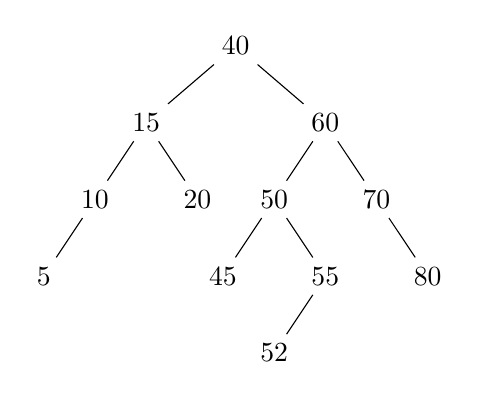
\begin{tikzpicture}[ level distance=1.5cm,
        level 1/.style={sibling distance=3.5cm},
        level 2/.style={sibling distance=2cm}, scale=.65]
            \node {40}
                child{node{15}
                        child{node{10} child{node{5}} child{node{} edge from parent
            [draw=none]}}
                        child{node{20}}}
                child{node{60}
                        child{node{50}
                                child{node{45}}
                                child{node{55}
                                        child{node{52}}
                                        child{node{} edge from parent [draw=none]}
                                }
                                }
                        child{node{70} child{node{} edge from parent [draw=none]}
                                child{node{80}}}
            };
    \end{tikzpicture}
    \end{center}
\begin{remark} Go over the properties and calculate the tree's height. Make sure you understand the definitions!
\end{remark}

Last time, we saw some operations that can be performed on BSTs, and
proved correctness for some of them. These were: $Search(x), Min(T), Max(T), Pred(x), Succ(x),
Insert(x), Delete(x)$. All of these operations take $O(h(T))$ in the worst case.\\

The main two operations that may cause problems are $Insert$ and $Delete$, as
they change the tree's height (consider inserting $81,82,83,84$ to our
working example).
To address this problem, we introduce another field: for each node $v$, add a field of $h(v)$ = the height of the subtree whose root is $v$. This allows us to maintain the AVL property:
\begin{defbox}{AVL Tree.} An AVL tree is a balanced BST, such that for any node $x$, its left and right subtrees' height differs in no more than $1$. In other words:
        $$|h(left(x)) - h(right(x))|\leq 1$$
    \end{defbox}
    This field allows us to calculate the Balance Factor for each node in $O
    (1)$:
    \begin{defbox}{Balance Factor.} For each node $x\in T$, it's Balance Factor is defined 
    $$hd
    (x) := h(left(x)) - h(right(x))$$ In AVL trees, we would like to maintain
    $|hd(x)| \leq 1$
    \end{defbox}
\begin{example} For our working example, the node $60$'s $hd$ is $h(50) - h
(70) = 1$, and $hd(50) = h(45)- h(55) = -1$. You can check and see that this is an AVL tree.
\end{example}
So to make sure that we can actually maintain time complexity $O(\log(n))$, we would want to:
\begin{enumerate}
    \item Show that for an AVL tree, $h(T) = \theta(log(n))$ (If there's time
    left)
    \item See how to correct violations in AVL property - using \textbf{rotations}
    \item See how to $Delete$ and $Insert$, while maintaining the height field.
\end{enumerate}

%\newpage
\subsection{Rotations}
\begin{figure}[h]
  \centering
\includegraphics[scale=.3]{Recitations/rotations.png}\\
\end{figure}
Rotations allow us to maintain the AVL property in $O(1)$ time (you have
discussed this in the lecture - changing subtree's roots).
In
this
schematic
representation of rotations, $x,y$ are nodes and $\alpha,\beta,\gamma$ are subtrees.
Note that the BST property is maintained! \\

%\includegraphics[scale=.5]{Recitations/rotationEg.png}

The Balance factor allows us to identify if the AVL property was violated, and moreover -
the exact values of the bad Balance factors will tell us which rotations to do to fix
this:\\
Taken from last year's recitation:\\
\includegraphics[scale=.6]{Recitations/violations.png}

Let us analyze one of these cases:\\
\begin{example} Let us see why R rotation Fixes LL violation:\\
\begin{figure}[h]
  \centering
\includegraphics[scale=.5]{Recitations/LLviolation.jpg}\\
This is the general form of LL violations.
\end{figure}

Let us analyze the heights of subtrees. Denote $h$ the height of $A_L$ before inserting $v$. So $A_R$'s height has also to be $h$.
If its height were $h+1$, the insertion would not have created a violation in
$B$ ($A$'s height would have stayed the same). If it were $h-1$, the violation would have appeared first in $A$ (not in $B$). Thus, $A$'s height is $h+1$.
$B_R$'s height is also $h$: If it was $h+1$ or $h+2$, no violation in $B$ had
occurred.

After the rotation, the tree looks like this:
\begin{figure}[h]
  \centering
  \includegraphics[scale=.9]{Recitations/LLviolationfix.jpg}
\end{figure}
So all the nodes here maintain AVL property; why is it maintained?
\end{example}\\
Detect the violation in the following tree, and perform the necessary rotations:\\
\begin{figure}[h]
  \centering
  \begin{subfigure}[b]{0.31\textwidth}
            \begin{tikzpicture}[ level distance=1.5cm,
        level 1/.style={sibling distance=3.5cm},
        level 2/.style={sibling distance=2cm}, scale=.65]
            \node {15}
	    child{node{5} child{node{3}} child{node{12}  child{node{10}
            child{node{6}} child{node{} edge from parent [draw = none]}}
            child{node{13}}}} child{node{20} child{node{18}} child{node{23}}}
            ;
    \end{tikzpicture}
  \end{subfigure}
\begin{subfigure}[b]{0.31\textwidth}
        \begin{tikzpicture}[ level distance=1.5cm,
        level 1/.style={sibling distance=3.5cm},
        level 2/.style={sibling distance=2cm}, scale=.65]
            \node {15}
	    child{node{} child{node{3}} child{node{10}
            child{node{6}} child{node{12} child{node{} edge
            from parent [draw = none]} child{node{13}} }}
            }
             child{node{20} child{node{18}} child{node{23}}}
            ;
    \end{tikzpicture}
  \end{subfigure}
\begin{subfigure}[b]{0.31\textwidth}
  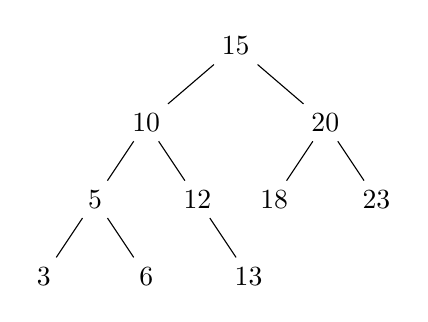
\begin{tikzpicture}[ level distance=1.5cm,
        level 1/.style={sibling distance=3.5cm},
        level 2/.style={sibling distance=2cm}, scale=.65]
            \node {15}
                child{node{10} child{node{5} child{node{3}} child{node{6}}
            } child{node{12}
            child{node{} edge from parent [draw = none]} child{node{13}}}}
             child{node{20} child{node{18}} child{node{23}}}
            ;
    \end{tikzpicture}

\end{subfigure}
  \caption{ 
The first node in which a violation occurred is $5$, this is an RL violation.
Perform R rotation on the right child. Then perform L rotation on the root of the relevant subtree ($5$):
}
\end{figure}
\subsection{Delete, Insert.}
The principles of the $Delete$ and $Insert$ operations are the same as in
regular BST, but we will need to rebalance the tree in order to preserve AVL
property.
A single insertion or deletion may change the height difference of subtrees
by at most 1, and might affect only the subtrees with roots along the path
from $r$ to the point of insertion/ deletion.
More concretely - we will add a recursive operation of traversing the tree
"back up" and checking violations. Had we found one - we will fix it using
rotations. Since rotations can be done in $O(1)$, the entire correction
process will take $O(\log(n))$, so we maintain a good time complexity.


\begin{algbox}{AVL Insert(r,x)}
  \begin{algorithm}[H]
    Call Insert $(r,x)$ // (The standard insertion routine for BST) \\  
    Let $p$ be the new node appended to the tree. \\
    \While{ $p$.parent $\neq \emptyset $ } {
      Check which of the four states we are in.\\ 
      Apply the right rotation. \\ 
      Update the height of each touched vertex  \\
      $p \leftarrow$ $p$.parent \\  
    }
  \end{algorithm}
\end{algbox}


\iffalse
\newpage
\subsection{Delete, Insert}
The principles of the $Delete$ and $Insert$ operations are the same as in
regular BST, but we will need to rebalance the tree in order to preserve AVL
property.
A single insertion or deletion may change the height difference of subtrees
by at most 1, and might affect only the subtrees with roots along the path
from $r$ to the point of insertion/ deletion.
More concretely - we will add a recursive operation of traversing the tree
"back up" and checking violations. Had we found one - we will fix it using
rotations. Since rotations can be done in $O(1)$, the entire correction
process will take $O(\log(n))$, so we maintain a good time complexity.
\subsubsection{Delete}
This is the regular BST delete. We will need to traverse up the
tree and detect violations (if occurred).\\
\includegraphics[scale=.6]{Recitations/DeleteBST.jpg}\\
\begin{remark} Go over the procedure quickly - explain the 3 cases - no
children, one child (easy), and two children (using successor).
\end{remark}
\begin{example}\\
    Delete $20$ from the tree at the beginning of the recitation:\\
    \includegraphics[scale=.3]{Recitations/DeleteEx.jpg}
\end{example}
%    Consider the original BST we looked at:\\
%
%\begin{tikzpicture}[ level distance=1.5cm,
%        level 1/.style={sibling distance=3.5cm},
%        level 2/.style={sibling distance=2cm}, scale=.65]
%            \node {40}
%                child{node{15}
%                        child{node{10} child{node{5}} child{node{} edge from parent
%            [draw=none]}}
%                        child{node{20}}}
%                child{node{60}
%                        child{node{50}
%                                child{node{45}}
%                                child{node{55}
%                                        child{node{52}}
%                                        child{node{} edge from parent [draw=none]}
%                                }
%                                }
%                        child{node{70} child{node{} edge from parent [draw=none]}
%                                child{node{80}}}
%            };
%    \end{tikzpicture}
%
%Let's $Insert(4)$:\\
%
%\begin{tikzpicture}[ level distance=1.5cm,
%        level 1/.style={sibling distance=3.5cm},
%        level 2/.style={sibling distance=2cm}, scale=.65]
%            \node {40}
%                child{node{15}
%                        child{node{(-2)10} child{node{(-1)5}child{node{4}}
%            child{node{} edge
%            from
%            parent
%            [draw = none]} }
%            child{node{} edge from
%            parent
%            [draw=none]}}
%                        child{node{20}}}
%                child{node{60}
%                        child{node{50}
%                                child{node{45}}
%                                child{node{55}
%                                        child{node{52}}
%                                        child{node{} edge from parent [draw=none]}
%                                }
%                                }
%                        child{node{70} child{node{} edge from parent [draw=none]}
%                                child{node{80}}}
%            };
%    \end{tikzpicture}\\
%
%So we need to fix LL violation. This is by performing R rotation of the root
%of the subtree in which the violation first appeared: \\
%
%\begin{tikzpicture}[ level distance=1.5cm,
%        level 1/.style={sibling distance=3.5cm},
%        level 2/.style={sibling distance=2cm}, scale=.65]
%            \node {40}
%                child{node{15}
%                        child{node{(0)5} child{node{(0)4}} child{node{10}}
%             }
%                        child{node{20}}}
%                child{node{60}
%                        child{node{50}
%                                child{node{45}}
%                                child{node{55}
%                                        child{node{52}}
%                                        child{node{} edge from parent [draw=none]}
%                                }
%                                }
%                        child{node{70} child{node{} edge from parent [draw=none]}
%                                child{node{80}}}
%            };
%    \end{tikzpicture}
%\begin{remark}
%    RR rotations are symmetric
%\end{remark}
\subsubsection{Insert}
Once again - this is the regular BST insert; we will need to traverse up the
tree and detect violations (if occurred).\\
\includegraphics[scale=.6]{Recitations/InsertBST.jpg}\\
\begin{example}
    Insert $65$ tho the previous tree (after the deletion):\\
    \begin{tikzpicture}[ level distance=1.5cm,
        level 1/.style={sibling distance=3.5cm},
        level 2/.style={sibling distance=2cm}, scale=.65]
            \node{50} child{node{40} child{node{10} child{node{5}
            }child{node{15}}} child{node{45}}}
            child{node{60} child{node{55}
                                    child{node{52}} child{node{} edge from
                                                            parent [draw=none]}}
                                    child{node{70}
                                            child{node{} edge from parent
            [draw=none]} child{node{80}}}}

    \end{tikzpicture}\\
    So after the insertion:\\
        \begin{tikzpicture}[ level distance=1.5cm,
        level 1/.style={sibling distance=3.5cm},
        level 2/.style={sibling distance=2cm}, scale=.65]
            \node{50} child{node{40} child{node{10} child{node{5}
            }child{node{15}}} child{node{45}}}
            child{node{60} child{node{55}
                                    child{node{52}} child{node{} edge from
                                                            parent [draw=none]}}
                                    child{node{70}
                                            child{node{65}} child{node{80}}}}

    \end{tikzpicture}\\
    And no violation occurred.\\
    \newpage
\end{example}
\begin{example}
    Insert 53 to the previous tree:\\
    \begin{tikzpicture}[ level distance=1.5cm,
        level 1/.style={sibling distance=3.5cm},
        level 2/.style={sibling distance=2cm}, scale=.65]
            \node{50} child{node{40} child{node{10} child{node{5}
            }child{node{15}}} child{node{45}}}
            child{node{60} child{node{55}
                                    child{node{52} child{node{} edge from
            parent [draw=none]} child{node{53}}} child{node{}
            edge
            from
                                                            parent [draw=none]}}
                                    child{node{70}
                                            child{node{65}} child{node{80}}}}

    \end{tikzpicture}\\
    Detect LR violation in $55$: Perform $L$ rotation on $52$:\\
    \begin{tikzpicture}[ level distance=1.5cm,
        level 1/.style={sibling distance=3.5cm},
        level 2/.style={sibling distance=2cm}, scale=.65]
            \node{50} child{node{40} child{node{10} child{node{5}
            }child{node{15}}} child{node{45}}}
            child{node{60} child{node{55}
                                    child{node{53} child{node{52}}
            child{node{} edge from parent[draw=none]}}
            child{node{}
            edge
            from
                                                            parent [draw=none]}}
                                    child{node{70}
                                            child{node{65}} child{node{80}}}}

    \end{tikzpicture}\\
    perform $R$ rotation on $55$:\\
    \begin{tikzpicture}[ level distance=1.5cm,
        level 2/.style={sibling distance=3cm},
        level 1/.style={sibling distance=5cm},
        level 3/.style={sibling distance=1.5cm},scale=.65]
            \node{50} child{node{40} child{node{10} child{node{5}
            }child{node{15}}} child{node{45}}}
            child{node{60} child{node{53}
                                    child{node{52}}
            child{node{55}}}
                                    child{node{70}
                                            child{node{65}} child{node{80}}}}

    \end{tikzpicture}\\

\end{example}

\newpage
\fi
\subsection{Exam Question.}
Consider the following question from 2018 exam. 
\begin{figure}[h]
  \centering
  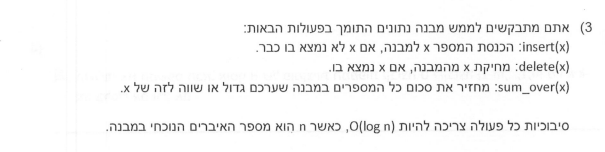
\includegraphics[scale=0.8]{avl-q-exam.png}\\
\end{figure}



\begin{figure}[H]
  \begin{subfigure}[b]{0.47\textwidth}
    \paragraph{Solution.} 

How would it look like an algorithm which computes the 'sum over' query? Or for given $x$, which vertices have a key less than $x$? 
Consider the path $v_1,v_2,v_3...v_n$ on which the Search subroutine went over when looking for $x$. If $v_i$.key $ <  v_{i+1}$.key then it means that $x$ is 
greater then $v_{i}$.key. Furthermore, $x$ is also greater than all the keys in the left subtree of $v_{i}$.

\paragraph{}

Let us transform that insight into an 
Algorithm. Define for each vertex a field that stores the summation of all its left subtree keys plus its own key; call it 'Leftsum'.  
Then computing the sumover query will be done by summing these fields of the vertices in the right turn on the searching path. 
\end{subfigure} 
\hfill
\begin{subfigure}[b]{0.49\textwidth}
  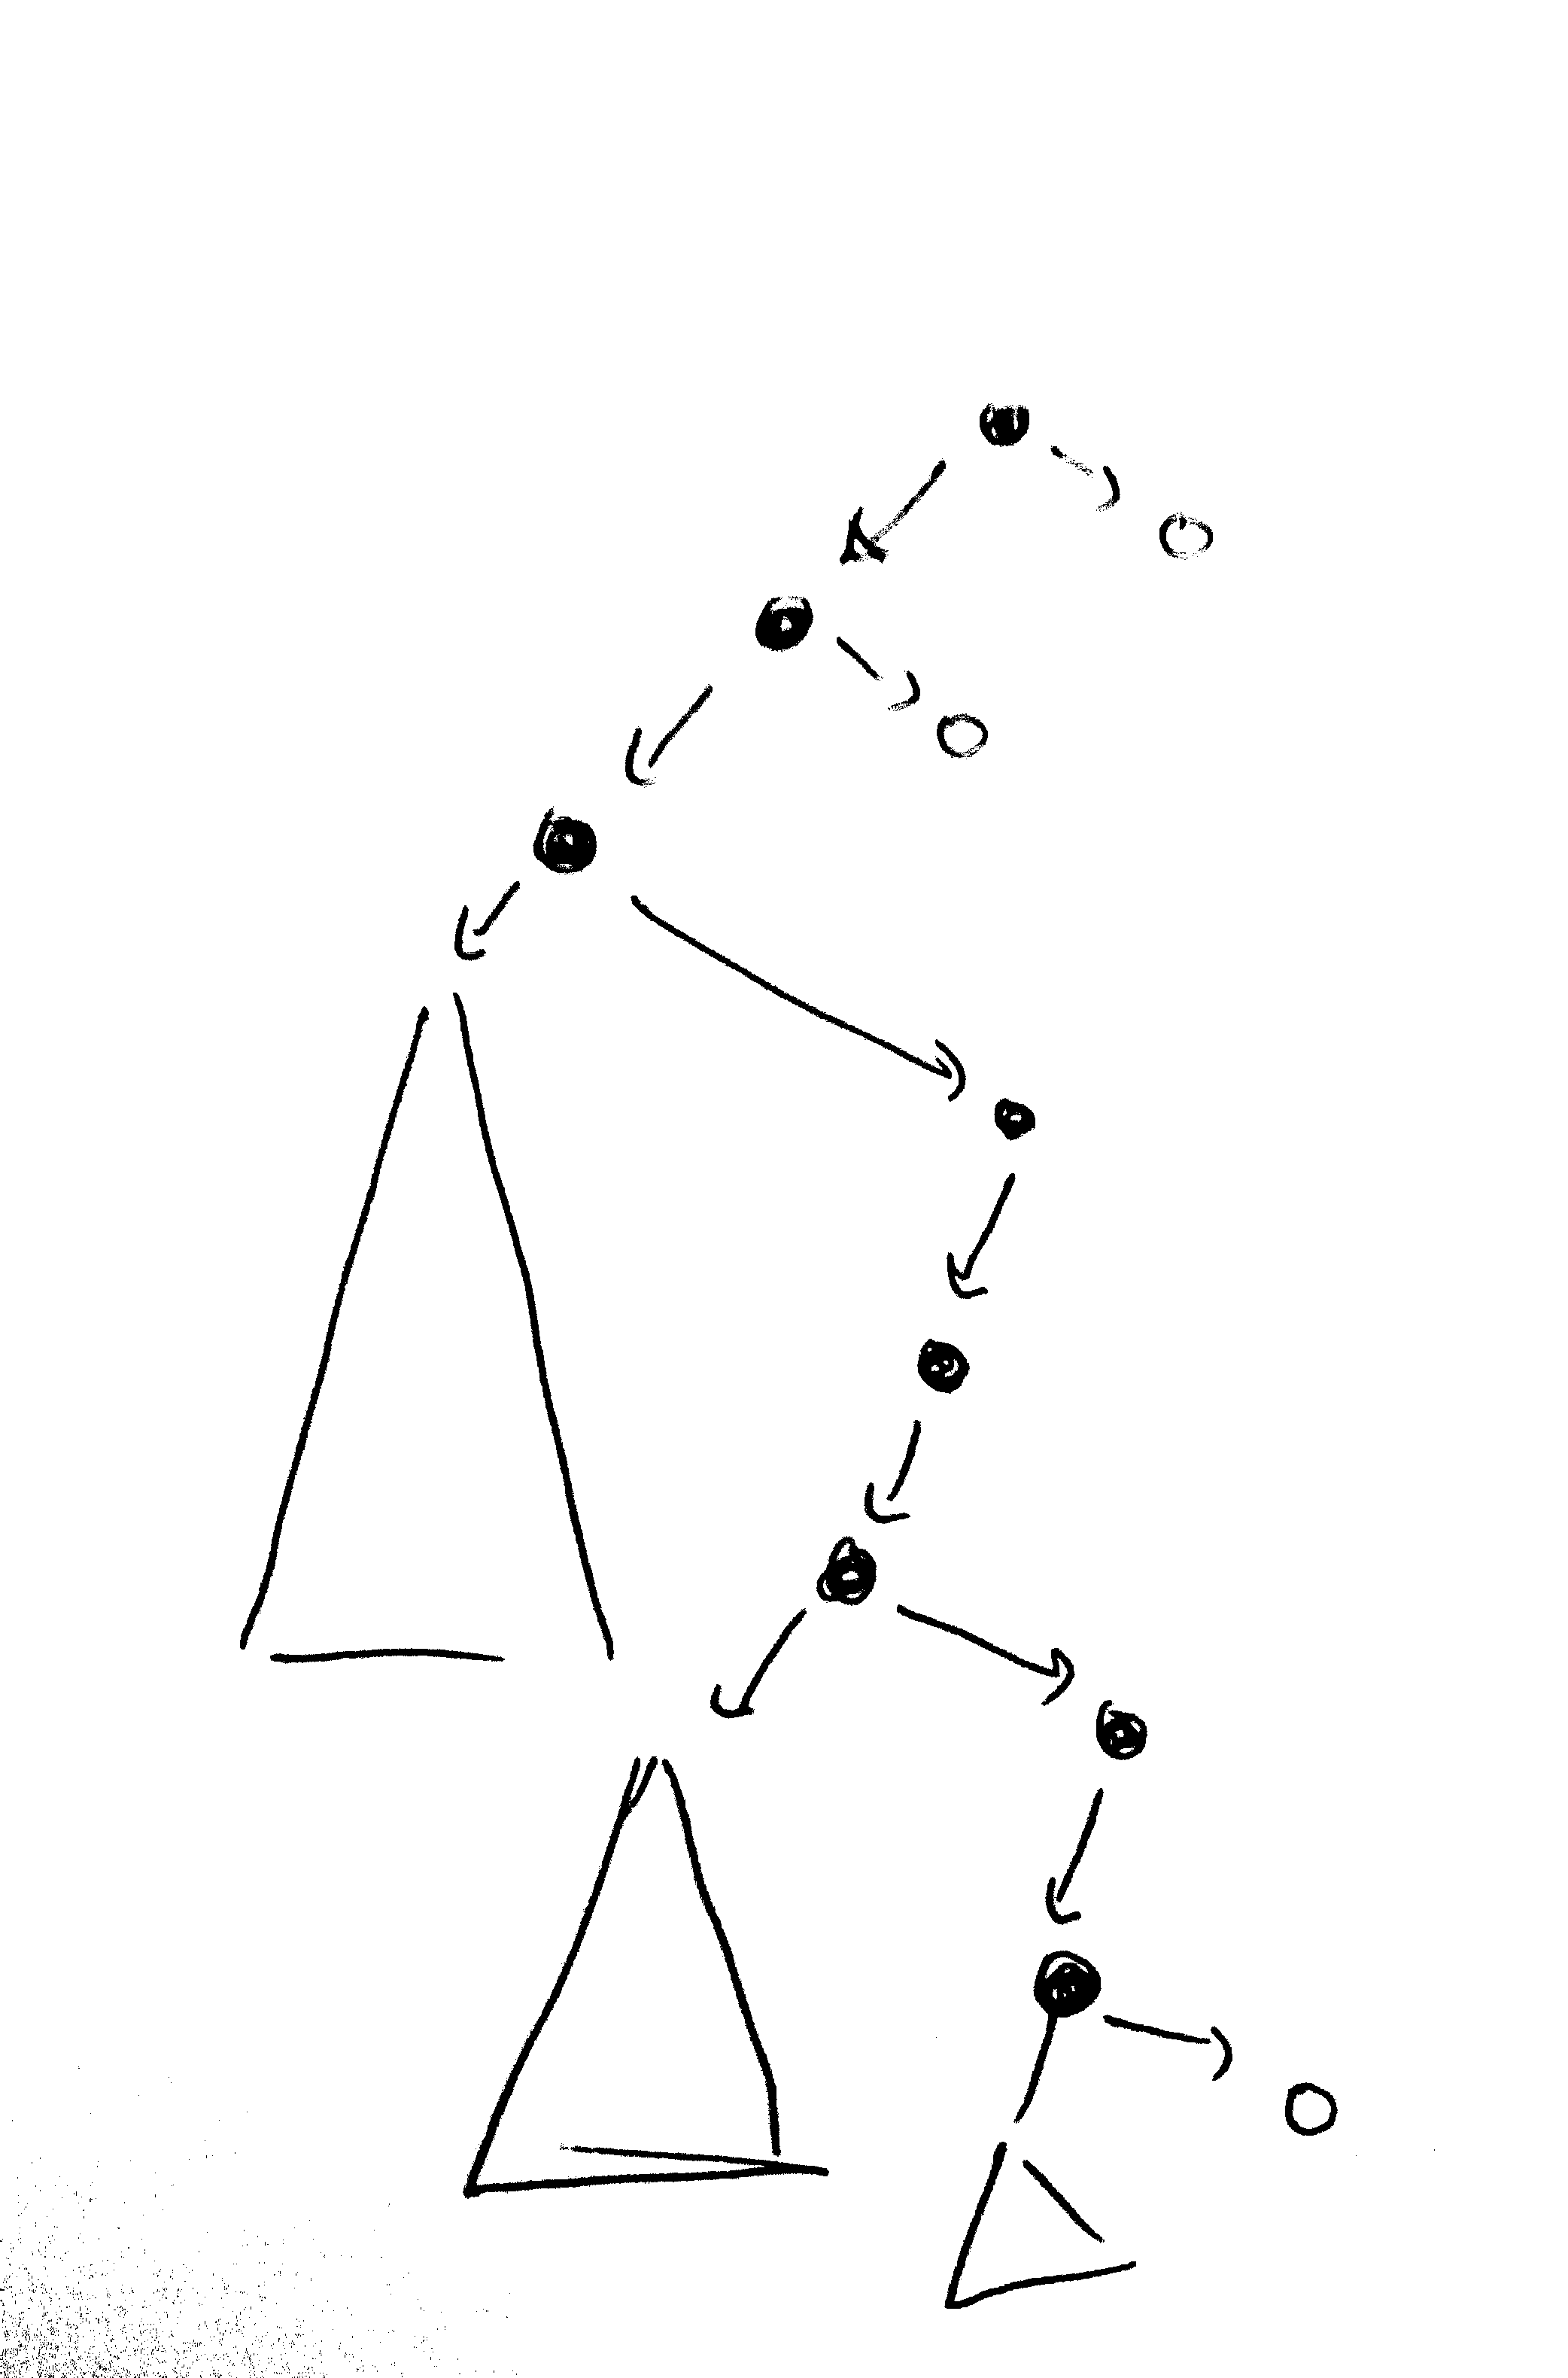
\includegraphics[scale=0.07]{oavl-q.png}
   \end{subfigure} 
   \hfill
\end{figure}


\begin{algbox}{Sumover($r$,$x$)}
  \begin{algorithm}[H]
    \If{ $r$ is None }{
      return $0$ 
    }\Else{
      \If{$x > r$.key }{
	return $r$.Leftsum + Sumover( $r$.right, $x$ )  
      }\Else{
      	return Sumover( $r$.left, $x$ )  
      }
    }
  \end{algorithm}
\end{algbox}

So it has left to show how one could maintain the tree and guarantee a logarithmic height. Consider a vertex $v$ and suppose that both
his direct children are correct AVL trees and have the correct value at the Leftsum field. We know that:
\begin{enumerate}
  \item There is a rotation that balances the tree at the cost of $O(1)$ time.
  \item All the descendants of $v$, at a distance at least two from it,  will remain the same in the sense that their subtree has not changed. 
\end{enumerate}
Therefore we will have to recompute the Sumleft filed for only a $O(1)$ vertices (which are the children and the grandchildren of $v$ previews the rotation). 
Each computation could be done in $O(1)$ time. 


\begin{algbox}{AVL-Leftsum Insert(r,x)}
  \begin{algorithm}[H]
    Call Insert $(r,x)$ // (The standard insertion routine for BST) \\  
    Let $p$ be the new node appended to the tree. \\
    \While{ $p$.parent $\neq \emptyset $ } {
      Apply the right rotation. \\
      \For{ any vertex $v$ such that its pointers have changed, sorted by height } {
	$v$.Leftsum $\leftarrow$ $v$.key + $v$.left.Leftsum + $v$.left.right.Leftism 		
      }
      $p \leftarrow$ $p$.parent \\  
    }
  \end{algorithm}
\end{algbox}

\paragraph{Running time.} The work is done over vertices along a single path, and on each vertex only $O(1)$ time 
is spent, Then we have that the total running time of the algorithm is proportional to the tree height. 
Combining the fact that we maintain the AVL property, it follows that the total time is $\Theta\left( \log n \right)$.  




\section*{Appendix}
\subsection{AVL tree's height}
Let $n_h$ be the minimal number of nodes in an AVL tree of height
$h$.\\
\begin{thm}
    $n_h$ is strictly increasing in $h$.
\end{thm}
\begin{proof} Exercise.
\end{proof}
\begin{thm}
$n_{h} = n_{h-1} + n_{h-2} + 1$.
\end{thm}
\begin{proof}For an AVL tree of height $0$, $n_0 = 1$,
and of height $1$, $n_1 = 2 $ (by checking directly).\\
    Let's look at a minimal AVL tree of height $h$. By the AVL property, one
of its subtrees is of height $h-1$ (WLOG - the left subtree) and by
minimality, its left subtree has to have $n_{h-1}$ nodes. $T$'s right subtree
thus has to be of height $h-2$: It can't be of height $h-1$: $n_{h-1} >
n_{h-2}$ by the previous theorem, and if the right subtree is of height $h-1$ -
we could switch it with an AVL tree of height $h-2$, with fewer nodes - so
less nodes in $T$, contradicting minimality. So the right subtree has
$n_{h-2}$ nodes (once again, by minimality), and thus the whole tree has
    $n_{h} = n_{h-1} + n_{h-2} + 1$ (added the root) nodes.
\end{proof}
\begin{cor}$n_h > 2n_{h-2} + 1$
\end{cor}
\begin{cor}$h = O(\log(n))$
\end{cor}
\begin{proof}
    Assume $k$ is even (why can we assume that?).
    It can be shown by induction that:
    \[
        n_h>2n_{h-2}+1>2(2n_{h-4}+1)+1=4n_{h-4}+(1+2)\ldots >
        2^{\frac{h}{2}}+\sum_{i=0}^{\frac{h}{2}-1}
        2^i=\sum_{i=1}^{\frac{h}{2}}2^i = \frac{2^\frac{h}{2} - 1}{2-1} =  2^{\frac{h}{2}} - 1
    \]
    So $n_h \geq 2^{\frac{h}{2}} - 1$, thus
    \[
        h\leq 2\log(n_h + 1)
    \]
    and for generall AVL tree with $n$ nodes and height $h$:
    \[
         h\leq 2\log(n_h + 1) \leq 2\log(n + 1) = O(\log(n))
    \]
%    By $n_h$'s minimality:
%    $$n \geq n_h \geq F_h = C (\varphi^h - (-\varphi)^h) \geq
%    \tilde{C}\varphi^h$$
%    Thus
%    $h \leq \frac{1}{\tilde{C}} \log_{\varphi}(n)$
\end{proof}
\begin{remark}
    In fact, one can show that $n_h > F_h$ and $F_h$ is the $h$'th Fibonacci
    number. Recall that $F_h = C(\varphi^h - (\psi)^h)$, and this gives a
    tighter bound on $n_h$.
\end{remark}

% \printbibliography 
\end{document}
\newpage